% !TeX encoding = UTF-8
% !TeX program = xelatex
% !TeX spellcheck = en_US

\documentclass[degree=postdoc]{thuthesis}
  % 学位 degree:
  %   doctor | master | bachelor | postdoc
  % 学位类型 degree-type:
  %   academic(默认)| professional
  % 语言 language
  %   chinese(默认)| english
  % 字体库 fontset
  %   windows | mac | fandol | ubuntu
  % 建议终版使用 Windows 平台的字体编译


% 论文基本配置,加载宏包等全局配置
% !TeX root = ./thuthesis-example.tex

% 论文基本信息配置

\thusetup{
  %******************************
  % 注意:
  %   1. 配置里面不要出现空行
  %   2. 不需要的配置信息可以删除
  %   3. 建议先阅读文档中所有关于选项的说明
  %******************************
  %
  % 输出格式
  %   选择打印版(print)或用于提交的电子版(electronic),前者会插入空白页以便直接双面打印
  %
  output = print,
  % 格式类型
  %   默认为论文(thesis),也可以设置为开题报告(proposal)
  % thesis-type = proposal,
  %
  % 标题
  %   可使用“\”命令手动控制换行
  %
  title  = {自动驾驶场景重建中的模型训练及渲染技术研究},
  title* = {Research on Model Training and Rendering Techniques for Reconstruction in Autonomous Driving Scenarios},
  %
  % 学科门类
  %   1. 学术型
  %      - 中文
  %        需注明所属的学科门类,例如:
  %        哲学、经济学、法学、教育学、文学、历史学、理学、工学、农学、医学、
  %        军事学、管理学、艺术学
  %      - 英文
  %        博士:Doctor of Philosophy
  %        硕士:
  %          哲学、文学、历史学、法学、教育学、艺术学门类,公共管理学科
  %          填写“Master of Arts“,其它填写“Master of Science”
  %   2. 专业型
  %      直接填写专业学位的名称,例如:
  %      教育博士、工程硕士等
  %      Doctor of Education, Master of Engineering
  %   3. 本科生不需要填写
  %
  % 博士后报告不需要学位类别
  % degree-category  = {工学硕士},
  % degree-category* = {Master of Science},
  %
  % 培养单位
  %   填写所属院系的全名
  %
  department = {计算机科学与技术系},
  %
  % 学科
  %   1. 研究生学术型学位,获得一级学科授权的学科填写一级学科名称,其他填写二级学科名称
  %   2. 本科生填写专业名称,第二学位论文需标注“(第二学位)”
  %
  discipline  = {计算机科学与技术},
  discipline* = {Computer Science and Technology},
  %
  % 专业领域
  %   1. 设置专业领域的专业学位类别,填写相应专业领域名称
  %   2. 2019 级及之前工程硕士学位论文,在 `engineering-field` 填写相应工程领域名称
  %   3. 其他专业学位类别的学位论文无需此信息
  %
  % professional-field  = {计算机技术},
  % professional-field* = {Computer Technology},
  %
  % 姓名
  %
  author  = {夏立斌},
  author* = {Xia Libin},
  %
  % 学号
  % 仅当书写开题报告时需要(同时设置 `thesis-type = proposal')
  %
  % student-id = {2000310000},
  %
  % 指导教师
  %   中文姓名和职称之间以英文逗号“,”分开,下同
  %
  supervisor  = {郑纬民, 教授},
  supervisor* = {Professor Zheng Weimin},
  %
  % 副指导教师
  %
  associate-supervisor  = {陈文光, 教授},
  associate-supervisor* = {Professor Chen Wenguang},
  %
  % 联合指导教师
  %
  % co-supervisor  = {某某某, 教授},
  % co-supervisor* = {Professor Mou Moumou},
  %
  % 日期
  %   使用 ISO 格式;默认为当前时间
  %
  % date = {2019-07-07},
  %
  % 是否在中文封面后的空白页生成书脊(默认 false)
  %
  include-spine = false,
  %
  % 密级和年限
  %   秘密, 机密, 绝密
  %
  % secret-level = {秘密},
  % secret-year  = {10},
  %
  % 博士后专有部分
  %
  clc                = {分类号},
  udc                = {UDC},
  id                 = {编号},
  discipline-level-1 = {计算机科学与技术},  % 流动站(一级学科)名称
  discipline-level-2 = {计算机应用技术},          % 专业(二级学科)名称
  start-date         = {2023-10-17},        % 研究工作起始时间
  end-date           = {2025-10-17},        % 研究工作期满时间
  postdoc-station    = {中国科学院深圳先进技术研究院},     % 流动站名称
  enterprise-mentor  = {朱福堂, 高级工程师},                     % 企业导师
  station-mentor     = {王琼, 研究员},                   % 流动站导师
  workstation-name   = {比亚迪汽车工业有限公司},              % 工作站/创新基地名称
  submission-date    = {2025-09-01},                      % 报告提交日期
  enterprise-department = {比亚迪汽车新技术研究院},                        % 企业部门
}

% 载入所需的宏包

% 定理类环境宏包
\usepackage{amsthm}
% 也可以使用 ntheorem
% \usepackage[amsmath,thmmarks,hyperref]{ntheorem}

\thusetup{
  %
  % 数学字体
  % math-style = GB,  % GB | ISO | TeX
  math-font  = none,  % stix | xits | libertinus | none
}

% Load unicode-math
\usepackage{unicode-math}
% Use default math font

% 可以使用 nomencl 生成符号和缩略语说明
% \usepackage{nomencl}
% \makenomenclature

% 表格加脚注
\usepackage{threeparttable}

% 表格中支持跨行
\usepackage{multirow}

% 固定宽度的表格。
% \usepackage{tabularx}

% 跨页表格
\usepackage{longtable}

% 算法
\usepackage{algorithm}
\usepackage{algorithmic}

% 量和单位
\usepackage{siunitx}

% 参考文献使用 BibTeX + natbib 宏包
% 顺序编码制
% \usepackage[sort]{natbib}
% \bibliographystyle{thuthesis-numeric}

% 著者-出版年制
% \usepackage{natbib}
% \bibliographystyle{thuthesis-author-year}

% 生命科学学院要求使用 Cell 参考文献格式(2023 年以前使用 author-date 格式)
% \usepackage{natbib}
% \bibliographystyle{cell}

% 本科生参考文献的著录格式
% \usepackage[sort]{natbib}
% \bibliographystyle{thuthesis-bachelor}

% 参考文献使用 BibLaTeX 宏包
% \usepackage[style=thuthesis-numeric]{biblatex}
% \usepackage[style=thuthesis-author-year]{biblatex}
\usepackage[style=gb7714-2015]{biblatex}
% \usepackage[style=apa]{biblatex}
% \usepackage[style=mla-new]{biblatex}
% 声明 BibLaTeX 的数据库
\addbibresource{ref/refs.bib}

% 定义所有的图片文件在 figures 子目录下
\graphicspath{{figures/}}

% 数学命令
\makeatletter
\newcommand\dif{%  % 微分符号
  \mathop{}\!%
  \ifthu@math@style@TeX
    d%
  \else
    \mathrm{d}%
  \fi
}
\makeatother

% hyperref 宏包在最后调用
\usepackage{hyperref}

% 加载 tcolorbox 包用于代码展示
\usepackage{tcolorbox}
\tcbuselibrary{skins,breakable}
\usetikzlibrary{calc}

% 加载 listings 包用于代码高亮
\usepackage{listings}

% 定义 tmpbox 环境用于代码展示
\newenvironment{tmpbox}{%
  \tcolorbox[%
  empty,
  parbox=false,
  noparskip,
  enhanced,
  % breakable,
  frame hidden,
  % boxrule=3pt %,
  colback=white,
  top = 1.2ex,
  bottom = 0.2ex,
  left=3ex, 
  % right=-4pt %,
  before skip=.5ex plus 2pt,
  after skip=1ex plus 2pt,
  overlay unbroken and last={%
    \draw ($(frame.north west)+(0.1, -2.0ex)$)
    -- +(0.985\textwidth, 0);
    \draw ($(frame.south west)+(0.1, 1.3ex)$)
    -- +(0.985\textwidth, 0);    
  }
  ]
}{\endtcolorbox}



\begin{document}

% 封面
\maketitle

% 学位论文指导小组、公开评阅人和答辩委员会名单
% 本科生不需要
\input{data/committee}

% 使用授权的说明
% 本科生开题报告不需要
\copyrightpage
% 将签字扫描后授权文件 scan-copyright.pdf 替换原始页面
% \copyrightpage[file=scan-copyright.pdf]

\frontmatter
% !TeX root = ../thuthesis-example.tex

% 中英文摘要和关键字

\begin{abstract}
  随着自动驾驶技术向L5级完全自主驾驶演进,高保真场景重建已从辅助感知工具转变为支撑整个研发体系的核心技术基础。在大规模仿真测试体系中,视点外推能力是实现灵活轨迹规划和多样化场景评估的关键技术瓶颈。现有神经场景表示方法在处理训练视点分布之外的新视角渲染时,普遍面临几何一致性退化和视觉质量下降的系统性问题。本文针对4D高斯溅射(4D Gaussian Splatting, 4DGS)在视点泛化能力上的根本性局限,提出了一种基于扩散先验的引导优化框架ReGen,通过系统性地融合视频扩散模型的生成先验知识来增强4DGS在未见视点上的渲染质量和几何一致性。

  本文的技术贡献体现在方法论创新、架构设计和系统实现三个层面。在方法论创新层面,提出了训练自由引导(Training-Free Guidance)机制,该机制通过同时利用LiDAR几何条件和当前4DGS渲染状态构建双重引导策略,将扩散模型的去噪过程显式地分解为条件引导和自由引导两个正交分量,实现了更加精确和稳定的监督信号传递。设计了自适应采样调度(Adaptive Sampling Scheduling)算法,根据4DGS模型的收敛状态和渲染质量动态调整扩散采样的频率和去噪强度,在训练早期提供强引导以建立正确的几何结构,在训练后期减弱引导以保持模型的泛化能力,显著提升了训练效率和优化质量。构建了多模态正则化框架,综合考虑几何一致性、时间连贯性和视觉质量三个维度,通过深度一致性正则项、光流平滑性约束和感知损失的协同作用,确保4DGS在优化过程中保持多视角几何结构的全局一致性和时序动态的平滑连贯性。

  在架构设计层面,提出了五层解耦的系统架构,包含数据抽象层、几何表示层、神经渲染层、扩散推理层和扩散监督层。数据抽象层负责输入数据的统一格式化和预处理;几何表示层采用静态背景、动态物体和环境映射的三元组合表示,支持大规模城市级场景的高效建模;神经渲染层实现了tile-based光栅化引擎,通过GPU内存池管理和自适应排序优化实现超过100帧每秒的实时渲染;扩散推理层封装了基于DiT架构的视频扩散模型,集成了滑动窗口机制和键值缓存技术以支持长序列生成;扩散监督层协调两个模型的联合优化,实现了内存高效的异步计算流水线。这种分层设计降低了系统复杂度,支持组件级的独立优化和灵活替换,为大规模系统的工程实现提供了坚实的架构基础。

  在系统实现层面,采用了基于Wan2.2-I2V-A14B的Diffusion Transformer(DiT)架构。该架构通过混合专家(Mixture-of-Experts, MoE)机制实现了基于信噪比的自适应专家路由,高噪声专家负责整体布局和动态构建,低噪声专家专注于细节优化,显著提升了视频生成的质量和效率。针对长视频序列处理的内存挑战,设计了50\%重叠的滑动窗口策略和跨窗口键值缓存机制,在保持长程时空依赖建模能力的同时有效控制了显存占用。实现了融合FSDP(Fully Sharded Data Parallel)和Ulysses序列并行的分布式训练架构,通过参数分片、梯度压缩和动态负载均衡策略,支持在多GPU集群上进行大规模模型的高效训练。设计了多模式推理引擎,支持单GPU和多GPU两种部署方式,通过模型权重卸载、数据类型转换和批处理优化,实现了灵活的性能与资源权衡。

  由于内部数据涉及保密要求,本文使用公开数据集进行实验验证,在视点外推任务上相比现有最先进方法取得了显著的性能提升,同时保持了实时渲染的计算效率。系统性的消融实验验证了各个技术组件的有效性和必要性,定性分析展示了方法在复杂城市场景中的渲染质量和几何一致性。需要说明的是,为满足学术发表的公开性要求,论文中部分技术细节已进行适当处理。研究成果为高保真场景重建技术在自动驾驶仿真中的实际应用提供了完整的理论框架、系统架构和工程实现方案,对推动自动驾驶技术向L5级完全自主驾驶演进具有重要的理论意义和实用价值。

  % 关键词用"英文逗号"分隔,输出时会自动处理为正确的分隔符
  \thusetup{
    keywords = {自动驾驶, 场景重建, 4D高斯溅射, 视频扩散模型, 扩散监督训练, 视点外推},
  }
\end{abstract}

\begin{abstract*}
  As autonomous driving technology advances toward Level 5 full autonomy, high-fidelity scene reconstruction has evolved from a perception assistance tool to a core technical foundation supporting the entire development ecosystem. In large-scale simulation testing frameworks, novel view extrapolation capability represents a critical technical bottleneck for achieving flexible trajectory planning and diverse scenario evaluation. Existing neural scene representation methods universally face systematic challenges of geometric consistency degradation and visual quality deterioration when rendering novel viewpoints beyond the training view distribution. This dissertation addresses the fundamental limitations of 4D Gaussian Splatting (4DGS) in view generalization by proposing ReGen, a diffusion-prior-based guided optimization framework that systematically integrates the generative prior knowledge of video diffusion models to enhance 4DGS's rendering quality and geometric consistency at unseen viewpoints.

  The technical contributions of this work are manifested across three levels: methodological innovation, architectural design, and system implementation. At the methodological innovation level, we propose a Training-Free Guidance mechanism that constructs a dual-guidance strategy by simultaneously leveraging LiDAR geometric conditions and current 4DGS rendering states, explicitly decomposing the denoising process of the diffusion model into conditional guidance and free guidance as two orthogonal components, achieving more precise and stable supervision signal propagation. We design an Adaptive Sampling Scheduling algorithm that dynamically adjusts the frequency and denoising strength of diffusion sampling based on the convergence state and rendering quality of the 4DGS model, providing strong guidance in early training stages to establish correct geometric structures while reducing guidance in later stages to maintain model generalization capability, significantly improving training efficiency and optimization quality. We construct a multi-modal regularization framework that comprehensively considers three dimensions—geometric consistency, temporal coherence, and visual quality—ensuring that 4DGS maintains global consistency of multi-view geometric structures and smooth coherence of temporal dynamics during optimization through the synergistic effects of depth consistency regularization, optical flow smoothness constraints, and perceptual losses.

  At the architectural design level, we propose a five-layer decoupled system architecture comprising data abstraction, geometric representation, neural rendering, diffusion inference, and diffusion supervision layers. The data abstraction layer handles unified formatting and preprocessing of input data; the geometric representation layer adopts a tripartite composition of static backgrounds, dynamic objects, and environment mapping to support efficient modeling of large-scale city-level scenes; the neural rendering layer implements a tile-based rasterization engine achieving real-time rendering exceeding 100 frames per second through GPU memory pool management and adaptive sorting optimization; the diffusion inference layer encapsulates a DiT architecture-based video diffusion model, integrating sliding window mechanisms and key-value caching techniques to support long-sequence generation; the diffusion supervision layer coordinates joint optimization of both models, implementing a memory-efficient asynchronous computation pipeline. This layered design reduces system complexity, supports component-level independent optimization and flexible replacement, providing a solid architectural foundation for large-scale system engineering implementation.

  At the system implementation level, we adopt a Diffusion Transformer (DiT) architecture based on Wan2.2-I2V-A14B. This architecture achieves adaptive expert routing based on signal-to-noise ratios through Mixture-of-Experts (MoE) mechanisms, where high-noise experts handle overall layout and dynamics construction while low-noise experts focus on detail refinement, significantly improving video generation quality and efficiency. To address memory challenges in long video sequence processing, we design a 50\% overlapping sliding window strategy with cross-window key-value caching mechanisms, effectively controlling memory footprint while maintaining long-range spatiotemporal dependency modeling capabilities. We implement a distributed training architecture integrating FSDP (Fully Sharded Data Parallel) and Ulysses sequence parallelism, supporting efficient training of large-scale models on multi-GPU clusters through parameter sharding, gradient compression, and dynamic load balancing strategies. We design a multi-mode inference engine supporting both single-GPU and multi-GPU deployment modes, achieving flexible performance-resource trade-offs through model weight offloading, data type conversion, and batch processing optimization.

  Due to confidentiality requirements of internal data, we conduct experimental validation using publicly available datasets, achieving significant performance improvements in novel view extrapolation tasks compared to state-of-the-art methods while maintaining real-time rendering computational efficiency. Systematic ablation experiments validate the effectiveness and necessity of each technical component, while qualitative analyses demonstrate the method's rendering quality and geometric consistency in complex urban scenarios. It should be noted that certain technical details have been appropriately adapted to meet the public disclosure requirements for academic publications. The research outcomes provide a complete theoretical framework, system architecture, and engineering implementation solution for high-fidelity scene reconstruction technology in autonomous driving simulation applications, holding significant theoretical importance and practical value for advancing autonomous driving technology toward Level 5 full autonomy.

  % Use comma as separator when inputting
  \thusetup{
    keywords* = {Autonomous Driving, Scene Reconstruction, 4D Gaussian Splatting, Video Diffusion Model, Diffusion-Supervised Training, Novel View Synthesis},
  }
\end{abstract*}


% 目录
\tableofcontents

% 插图和附表清单(表在前,图在后)
\makeatletter
\clearpage
\phantomsection
\addcontentsline{toc}{chapter}{插图和附表清单}
\chapter*{插图和附表清单}
\@starttoc{lot}%
\par
\null\par
\@starttoc{lof}%
\makeatother

% 符号对照表
% !TeX root = ../thuthesis-example.tex

\begin{denotation}[4cm]
  % 缩写和专有名词
  \item[4DGS] 4D高斯溅射(4D Gaussian Splatting)
  \item[3DGS] 3D高斯溅射(3D Gaussian Splatting)
  \item[NeRF] 神经辐射场(Neural Radiance Fields)
  \item[SDS] 分数引导采样(Score Distillation Sampling)
  \item[DiT] 扩散变换器(Diffusion Transformer)
  \item[MoE] 混合专家(Mixture of Experts)
  \item[FSDP] 完全分片数据并行(Fully Sharded Data Parallel)
  \item[LiDAR] 激光雷达(Light Detection and Ranging)
  \item[RGB-D] 彩色深度图像(Red-Green-Blue-Depth)
  \item[SAM] 分割任意模型(Segment Anything Model)
  \item[SE(3)] 三维特殊欧氏群(3D Special Euclidean Group)
  
  % 损失函数相关
  \item[$\mathcal{L}_{\text{recon}}$] 重建损失(Reconstruction Loss)
  \item[$\mathcal{L}_{\text{novel}}$] 新视点监督损失(Novel View Supervision Loss)
  \item[$\mathcal{L}_{\text{depth}}$] 深度监督损失(Depth Supervision Loss)
  \item[$\mathcal{L}_{\text{sky}}$] 天空区域损失(Sky Region Loss)
  \item[$\mathcal{L}_{\text{scale}}$] 尺度正则化损失(Scale Regularization Loss)
  \item[$\mathcal{L}_{\text{temporal}}$] 时间一致性损失(Temporal Consistency Loss)
  \item[$\mathcal{L}_{\text{LPIPS}}$] 感知损失(Learned Perceptual Image Patch Similarity)
  \item[$\mathcal{L}_{\text{SSIM}}$] 结构相似性损失(Structural Similarity Loss)
  
  % 高斯参数
  \item[$\mathcal{G}$] 高斯基元集合(Gaussian Primitive Set)
  \item[$\boldsymbol{\mu}$] 高斯中心位置(Gaussian Mean Position)
  \item[$\boldsymbol{\Sigma}$] 高斯协方差矩阵(Gaussian Covariance Matrix)
  \item[$\alpha$] 高斯不透明度(Gaussian Opacity)
  \item[$\mathbf{s}$] 高斯尺度参数(Gaussian Scale Parameters)
  \item[$\mathbf{c}$] 高斯颜色(Gaussian Color)
  \item[SH] 球谐函数(Spherical Harmonics)
  
  % 扩散模型相关
  \item[$\epsilon_\theta$] 扩散模型噪声预测网络(Noise Prediction Network)
  \item[$\mathbf{C}_{\text{lidar}}$] LiDAR几何条件(LiDAR Geometric Condition)
  \item[$\mathbf{I}_{\text{pseudo}}$] 扩散生成的伪真值(Diffusion-generated Pseudo GT)
  \item[$\mathbf{I}_{\text{render}}$] 渲染图像(Rendered Image)
  \item[$s$] 引导强度(Guidance Scale)
  \item[$t$] 扩散时间步(Diffusion Timestep)
  
  % 渲染相关
  \item[$\mathcal{R}$] 渲染函数(Rendering Function)
  \item[$\pi$] 相机视点(Camera Viewpoint)
  \item[$\mathbf{K}$] 相机内参矩阵(Camera Intrinsic Matrix)
  \item[$\mathbf{T}_{w2c}$] 世界到相机变换(World-to-Camera Transform)
  \item[$D_{\text{render}}$] 渲染深度图(Rendered Depth Map)
  \item[$D_{\text{lidar}}$] LiDAR深度图(LiDAR Depth Map)
  
  % 场景表示相关
  \item[$\mathcal{G}_{\text{bkgd}}$] 静态背景高斯(Background Gaussians)
  \item[$\mathcal{G}_{\text{obj}}$] 动态物体高斯(Object Gaussians)
  \item[$\mathcal{G}_{\text{sky}}$] 天空高斯(Sky Gaussians)
  \item[$\mathcal{P}$] 点云(Point Cloud)
  \item[$\mathcal{B}$] 3D边界框(3D Bounding Box)
  
  % 训练相关
  \item[$\eta$] 学习率(Learning Rate)
  \item[$\tau_{\text{grad}}$] 梯度阈值(Gradient Threshold)
  \item[$\tau_{\text{scale}}$] 尺度阈值(Scale Threshold)
  \item[$\tau_{\text{opacity}}$] 不透明度阈值(Opacity Threshold)
  \item[$\lambda$] 损失权重系数(Loss Weight Coefficient)
  
  % 图像质量度量
  \item[PSNR] 峰值信噪比(Peak Signal-to-Noise Ratio)
  \item[SSIM] 结构相似性(Structural Similarity Index)
  \item[LPIPS] 感知相似性(Learned Perceptual Image Patch Similarity)
  \item[FPS] 帧率(Frames Per Second)
  
  % 其他
  \item[GPU] 图形处理器(Graphics Processing Unit)
  \item[CPU] 中央处理器(Central Processing Unit)
  \item[FP16] 16位浮点数(16-bit Floating Point)
  \item[Adam] 自适应矩估计优化器(Adaptive Moment Estimation)
\end{denotation}



% 正文部分
\mainmatter
% !TeX root = ../thuthesis-example.tex

\chapter{引言}

随着自动驾驶技术向L5级完全自主驾驶的演进,高保真场景重建已从辅助感知的工具转变为支撑整个自动驾驶研发体系的核心技术基础。在这一历史性转变过程中,传统的场景理解方法正面临前所未有的挑战,而新兴的神经场景表示技术则为突破这些瓶颈提供了新的可能。本章将从自动驾驶技术发展的宏观视角出发,深入分析高保真场景重建的战略价值,系统阐述神经场景表示技术的演进轨迹,重点探讨当前技术面临的核心挑战,并明确本论文的研究动机和主要贡献。

\section{高保真场景重建的战略意义与技术挑战}

自动驾驶技术的发展历程清晰地展现了从简单辅助驾驶到完全自主驾驶的技术演进路径。在这一演进过程中,场景理解技术的需求发生了根本性的变化。早期的L2和L3级别系统主要依赖于高度抽象化的环境表示方法,包括2D和3D边界框、车道线检测以及交通标志识别等符号化信息处理技术\cite{chen2025snerf}。这种稀疏化的场景表示方法在结构化程度较高的高速公路环境中表现相对可接受,但在面对复杂多变的城市驾驶场景时,其局限性变得日益明显。

L5级完全自主驾驶技术的核心挑战在于如何稳健地处理现实世界中的"长尾问题"。这些长尾场景包括但不限于恶劣天气条件下的驾驶、复杂交通状况的应对、基础设施异常情况的处理等。传统的数据驱动方法在面对这些罕见但安全关键的驾驶场景时,往往受到数据稀缺性和数据采集成本高昂的双重制约\cite{yan2024street}。据业界统计,要通过真实世界的道路测试来覆盖99.9\%的安全关键场景,需要累计行驶超过110亿英里的里程,这在经济成本和时间投入上都是难以承受的。

在这样的技术背景下,高保真场景重建技术的价值定位发生了战略性的转移。其角色已经从提升直接感知能力的辅助工具,转变为赋能大规模仿真测试的核心技术基础。这种根本性的转变对技术标准提出了更加严苛的要求。首先是几何精度要求的显著提升,需要从传统的厘米级精度提升到毫米级精度,以支持更加精确的碰撞检测和路径规划算法。其次是视觉保真度的大幅改善,需要从功能性表示提升到照片级真实感,以支持感知算法的闭环测试验证。此外,还需要具备良好的时间连贯性,能够从静态场景快照扩展到动态序列建模,以支持复杂驾驶行为的高保真仿真。最后,系统还必须具备强大的视点可控性,能够从固定视角的观测扩展到任意视点的渲染,以支持多样化驾驶策略的全面测试。

视点外推能力是高保真场景重建技术面临的最核心挑战之一。从技术本质上看,视点外推问题可以理解为在训练视点分布范围之外的新视点上进行高质量渲染的技术难题。这一挑战的根源在于几何表示方法的固有不完整性和有效先验知识的缺失。传统的显式表示方法,如点云和三角网格,在训练数据覆盖不到的空间区域往往缺乏有效的插值机制,而隐式表示方法虽然在理论上具有更好的插值能力,但其巨大的计算开销使其难以满足实时仿真应用的性能要求。

从信息论的角度来理解,视点外推问题本质上是一个条件生成问题,即如何在给定有限训练观测的条件下,对未见视点进行合理的场景内容推断。传统方法的主要局限在于其学习到的场景表示过于尖锐和特化,缺乏足够的泛化能力来处理训练分布之外的视点查询。这种局限性在实际应用中表现为渲染质量随视点偏离程度的急剧下降,严重制约了高保真仿真系统的实用价值。

\section{神经场景表示技术的演进与现状分析}

神经场景表示技术的发展历程体现了从隐式表示到显式表示的重要技术范式转变。Neural Radiance Fields(NeRF)作为隐式神经表示的典型代表,通过多层感知机网络学习连续的体积密度和辐射场函数,实现了前所未有的场景重建质量\cite{mildenhall2021nerf}。NeRF的核心创新在于将场景建模为一个连续的五维函数,该函数能够将三维空间位置和二维观测方向映射为体积密度和辐射颜色。这种连续函数表示的优势在于其天然的可微分性质,使得模型能够直接从二维图像监督中学习三维场景结构,无需额外的几何先验知识。

尽管NeRF在静态场景重建方面取得了突破性进展,但其在处理大规模动态场景时面临三个根本性的技术挑战。首先是计算复杂度问题,每个像素的渲染过程需要沿光线方向进行密集采样并执行大量的神经网络前向推理,导致渲染速度远远低于实时应用的要求。其次是可扩展性限制,单一神经网络的表达容量有限,难以有效表征广阔的城市级场景。虽然Block-NeRF和Mega-NeRF等方法通过空间分割策略在一定程度上缓解了这一问题,但也引入了模型管理复杂性和边界不连续性等新的技术挑战\cite{blocknerf2022,meganeRF2022}。第三个挑战是动态建模的困难,NeRF的静态场景假设与动态驾驶环境的本质需求存在根本性矛盾。

3D Gaussian Splatting(3DGS)的出现标志着神经场景表示技术从隐式到显式的重要范式转变\cite{kerbl2023gaussian}。3DGS采用显式的三维高斯基元集合来表示场景,每个高斯基元通过位置、协方差矩阵、不透明度和颜色等参数进行完整描述。这种显式表示的最大优势在于渲染效率的显著提升,通过可微分的点splatting技术,3DGS能够实现超过100帧每秒的实时渲染性能,为实际应用部署奠定了坚实的技术基础。

然而,3DGS在视点外推任务上存在根本性的技术局限。这种局限源于显式表示方法的本质特性:3DGS在训练过程中主要学习如何合理排布高斯基元,使其从训练视点观察时能够产生正确的视觉效果,但缺乏强大的几何或语义先验来约束全局场景的一致性。这导致模型容易对特定的训练视点分布产生过拟合现象。与NeRF的连续函数表示不同,3DGS的离散基元表示在训练数据覆盖不足的空间区域缺乏有效的插值机制,当查询视点远离训练分布时,容易出现几何不一致和明显的视觉伪影。

更为关键的是,3DGS缺乏关于真实世界场景结构的内在先验知识,无法在数据稀疏区域进行合理的场景内容补全。实验分析表明,3DGS的视点外推性能与视点偏离距离呈现明显的指数衰减关系,这种性能退化严重限制了其在需要广泛视点覆盖的仿真应用中的实用价值。

\section{扩散模型的生成先验与融合机遇}

扩散模型通过在大规模数据集上的预训练,已经内隐地学习了丰富的视觉先验知识\cite{ho2020denoising}。这些先验知识体现在模型对真实世界视觉模式的深度理解上,包括几何结构的合理性、光照效果的真实性、材质属性的一致性以及物理约束的遵循等多个方面。从贝叶斯学习的理论角度来看,扩散模型实际上学习了数据分布的梯度场,这种梯度场包含了关于数据分布结构的丰富信息,为指导三维场景的生成和优化提供了强大的理论基础。

分数蒸馏采样(Score Distillation Sampling, SDS)技术的提出为将二维扩散先验有效应用于三维内容生成提供了重要的理论框架\cite{dreamfusion2022}。SDS的核心思想是将预训练的二维扩散模型转化为可微分的损失函数,通过梯度反传的方式指导三维表示的优化过程。这种方法的理论优势在于能够将扩散模型学习到的丰富视觉先验直接迁移到三维场景重建任务中,为解决视点外推等关键技术挑战提供了新的思路。

将扩散模型的生成先验迁移到三维表示的过程本质上是一个知识蒸馏问题。在这个框架中,预训练的扩散模型充当教师网络的角色,为三维表示的学习提供高质量的监督信号。这种知识蒸馏范式的理论优势体现在三个方面:首先是先验知识的有效迁移,能够将扩散模型在大规模数据上学习到的视觉先验迁移到三维表示中;其次是泛化能力的显著增强,通过生成先验的引导,三维表示在未见视点上的表现能够得到明显改善;最后是效率与质量的良好平衡,既保持了三维表示的渲染效率优势,又提升了生成内容的视觉质量。

当前融合神经场景表示与生成模型的方法主要可以归纳为三种技术范式。数据机器范式通过离线生成额外的训练数据来改善模型性能,其代表性工作包括DriveDreamer4D等。在线修复范式将生成模型作为实时修复器嵌入训练循环,典型代表是ReconDreamer等方法。知识蒸馏范式采用两阶段的训练流程实现知识迁移,StreetCrafter等工作属于这一类别。每种范式都有其独特的技术优势,但也存在相应的局限性,为本论文的技术创新提供了明确的改进空间。

\section{研究动机与核心贡献}

基于对现有技术发展状况的深入分析,本论文的研究动机可以概括为三个层面的技术需求。首先是理论层面的需求,现有方法缺乏统一的理论框架来分析不同融合范式的优劣,对知识蒸馏过程的收敛性和稳定性也缺乏严格的理论保证。其次是算法层面的需求,现有的引导机制相对简单,无法充分利用多模态信息;采样策略缺乏自适应性,难以根据训练状态进行动态调整;正则化机制不够完善,难以有效平衡多个优化目标。最后是系统层面的需求,缺乏端到端的优化框架使得组件间的协同效应未能得到充分发挥,内存和计算效率有待提升,标准化的评估框架也亟待建立。

针对这些技术需求,本论文提出了一种改进的知识蒸馏框架,主要贡献体现在四个方面。第一个贡献是训练自由引导机制的设计,提出了一种新颖的引导策略,能够同时利用几何条件和当前渲染状态作为引导信号,实现更加精确和稳定的知识迁移过程。第二个贡献是自适应采样调度算法的开发,设计了基于训练状态感知的自适应采样调度机制,能够根据4DGS模型的收敛情况动态调整扩散采样的频率和强度,显著提升了训练效率和蒸馏质量。第三个贡献是多模态正则化框架的构建,提出了综合考虑几何一致性、时间连贯性和视觉质量的正则化体系,通过多个正则化项的协同作用确保蒸馏过程的稳定性和最终结果的质量。第四个贡献是分层系统架构的设计,构建了五层解耦的系统架构,实现了复杂算法的模块化分解和高效实现,为大规模系统的开发和维护提供了良好的技术基础。

这些技术贡献不仅在理论上具有创新性,更重要的是在实际应用中展现出显著的性能优势。通过系统性的实验验证,本论文提出的方法在视点外推任务上相比现有最先进方法取得了显著的性能提升,为高保真场景重建技术在自动驾驶仿真中的实际应用奠定了坚实的技术基础。

\section{论文组织结构}

本论文的组织结构遵循从理论分析到实践验证的逻辑脉络。第二章系统回顾相关工作,深入分析神经场景表示方法、扩散模型在三维生成中的应用以及两者融合的最新进展,为本文的技术贡献提供充分的背景铺垫和对比基准。第三章详细阐述本文提出的核心方法论,包括问题的数学形式化描述、可控视频扩散模型的设计原理、知识蒸馏框架的构建方法以及训练自由引导机制的理论分析。第四章介绍系统的架构设计和工程实现细节,涵盖分层架构的设计原理、高性能渲染引擎的实现方案、内存优化策略以及分布式训练的技术方案。第五章展示全面的实验结果和深入分析,包括在多个标准数据集上的定量和定性评估、详细的消融实验分析以及与现有方法的系统性对比。第六章总结全文的主要贡献,客观分析方法的局限性,并对未来的研究方向进行前瞻性展望。

% !TeX root = ../thuthesis-example.tex

\chapter{相关工作}

本章系统性地回顾与本论文研究方向密切相关的理论基础和技术发展脉络。自动驾驶系统的构建需要在动态环境中实现准确的感知、预测和决策\cite{chen2024autonomous,hu2023planning,ma2024vision,kong2025multimodal}。为了在规模化条件下开发和评估此类系统,能够合成多样化、逼真且时序一致的4D场景的驾驶仿真器正变得日益关键。然而,收集和标注大规模真实世界驾驶数据集既昂贵又耗时,通常受到传感器覆盖范围、天气条件、遮挡和场景多样性的限制。为解决这些局限性,生成模型作为一种前景广阔的替代方案应运而生,使得能够可控且可扩展地创建用于感知和规划任务的合成驾驶场景。

基于扩散的模型在高保真图像和视频生成方面取得了显著成功,并正在积极探索应用于城市场景仿真。本章将从三个维度展开深入分析:首先综述驾驶场景生成技术的发展,包括视频生成和4D场景生成方法;其次回顾场景重建技术的演进,特别关注基于3D高斯溅射的动态场景重建方法;最后介绍扩散强制技术的理论基础及其在视频生成中的应用,为本论文的技术创新提供理论支撑。

\section{驾驶场景生成技术}

近年来,基于扩散的方法\cite{ho2020denoising,ddpm2015,song2020score}已成为图像和视频生成领域的主导范式。基于这一成功,多项研究工作\cite{gao2024magicdrive,wen2024panacea,mao2025dreamdrive,wang2024drivedreamer,wang2024stag1,wen2024panacea,li2024hierarchical,gao2025vista,li2023bridging,wang2024driving}将扩散模型扩展到自动驾驶场景的生成和重建任务中。本节将从视频驾驶生成和4D驾驶生成两个层面系统性地分析该领域的技术进展。

\subsection{视频驾驶生成}

视频驾驶生成的核心目标是合成时序连贯且视觉逼真的街景视频序列。这一任务的挑战性在于需要同时满足多个约束条件:不仅要保证单帧图像的视觉质量,还要维持帧间的时序平滑性,同时响应各种控制信号如地图、轨迹和交通规则等。MagicDrive\cite{gao2024magicdrive}在这方面做出了开创性工作,通过编码多种3D几何信号作为条件输入,并采用跨视角注意力机制来增强帧间一致性,实现了高质量街景视频的生成。该方法的创新之处在于设计了多模态条件编码器,将BEV地图、3D边界框、实例掩码等结构化3D信息有效融入扩散过程的每一步,使得生成的视频能够在保持视觉真实性的同时维持几何一致性。此外,MagicDrive引入的跨视角注意力机制能够捕捉不同相机视角之间的空间关系,在一定程度上缓解了多视角不一致的问题。

在MagicDrive的基础上,后续工作进一步探索了提升时序连贯性和可控性的方法。Panacea\cite{wen2024panacea}提出了全景视频生成框架,其核心贡献在于设计了统一的潜在空间表示,能够同时控制多个视角的视频生成。该方法通过在潜在空间中共享全局场景表示,确保不同视角生成的视频在几何结构和语义内容上保持一致。这种设计使得系统能够生成360度环绕视角的连贯视频,为全方位场景理解提供了数据基础。DriveDreamer\cite{wang2024drivedreamer}则从另一个角度出发,构建了面向真实世界的世界模型。该方法不仅关注视频生成的视觉质量,更强调生成内容应符合真实世界的物理规律和交通规则。通过在大规模真实驾驶数据上学习场景的动态演化规律,DriveDreamer能够生成更加自然和合理的驾驶场景,包括车辆的加速减速、行人的移动模式、交通灯的变化等动态元素。

然而,这些视频生成方法存在一个根本性的局限:缺乏准确且连贯的3D空间表示。这一问题源于扩散模型本质上是在2D图像空间进行建模,虽然可以通过条件信号引入3D几何信息,但模型并不直接学习和维护完整的3D场景结构。因此,生成的视频虽然在单视角下具有较高的视觉质量,但往往无法保证多视角几何一致性。例如,当从不同视角观察同一场景时,可能出现物体位置不对应、尺度不一致、甚至几何结构矛盾等问题。这种几何不一致性在自动驾驶仿真中是不可接受的,因为感知算法和规划算法都依赖于精确的3D空间理解。

此外,现有视频生成方法通常与预定义的自车轨迹紧密耦合,只能生成沿着固定相机路径的视频序列。这种设计虽然简化了问题,但严重限制了系统的灵活性。在实际的自动驾驶仿真中,我们往往需要从任意视角观察场景,以评估感知系统在不同视角下的性能,或者可视化规划模块生成的多种可能轨迹。然而,这些视频生成方法无法支持新视角合成(Novel View Synthesis, NVS),一旦偏离训练时的相机分布,生成质量会急剧下降。这一局限性促使研究者们开始探索4D感知的场景生成方法,即不仅生成时序连贯的视频,还要构建完整的3D场景表示,以支持任意视角的渲染。

为了提升视频生成的时序连贯性和多视角一致性,一些工作从多个角度进行了深入探索\cite{li2024hierarchical,gao2025vista,li2023bridging,wang2024driving}。Li等人\cite{li2024hierarchical}提出了层次化时序上下文学习方法,其核心思想是在不同时间尺度上建模场景动态。该方法设计了多尺度的时序编码器,能够同时捕捉短期的局部运动(如车辆的瞬时速度变化)和长期的全局趋势(如整体交通流的演化)。通过这种层次化建模,系统能够生成在多个时间尺度上都保持连贯的视频序列。

VISTA\cite{gao2025vista}则着眼于构建通用的驾驶世界模型,目标是开发一个能够适应不同场景、不同天气条件、不同地理位置的统一生成框架。该方法通过在多样化的大规模数据集上进行训练,学习到了丰富的场景先验知识,包括道路结构、交通参与者的行为模式、光照变化等。VISTA的一个重要特点是其可控性,用户可以通过多种方式指定生成内容,如文本描述、轨迹规划、地图信息等。在多个基准测试中,VISTA展现了优异的泛化能力,能够生成在视觉质量和物理合理性上都接近真实数据的仿真场景。此外,Li等人\cite{li2023bridging}和Wang等人\cite{wang2024driving}分别从立体几何融合和多视角预测的角度,提出了提升几何一致性的新方法。

尽管这些工作从不同角度推动了视频驾驶生成技术的发展,但它们都未能从根本上解决3D几何一致性问题。其核心原因在于这些方法仍然是在2D视频空间进行生成,缺乏显式的3D场景表示作为约束。这促使研究者们转向4D场景生成方法,试图在生成过程中同时构建完整的3D几何结构。

\subsection{4D驾驶场景生成}

为了解决视频生成方法缺乏3D空间表示的问题,研究者们开始探索4D感知的场景生成方法。所谓4D生成,是指同时建模场景的三维空间结构和时间演化,生成包含完整几何信息的动态场景表示。与传统的2D视频生成相比,4D生成面临着更高的复杂度:不仅要求在时间维度上保持连贯性,还需要在三维空间中维持几何一致性,确保从任意视角渲染的结果都符合相同的3D结构。这一能力对于支持灵活的新视角合成至关重要,是构建高保真驾驶仿真器的必要条件。

4D场景生成的技术挑战是多方面的。首先是表示选择的问题:应该采用何种3D表示来同时满足几何准确性、渲染效率和生成灵活性的要求?其次是生成一致性的保证:如何确保生成的3D场景在不同视角和时刻都保持物理合理性和视觉连贯性?最后是计算效率的权衡:4D生成涉及的数据量和计算复杂度都远超2D视频生成,如何在可接受的计算成本下实现高质量的4D场景合成?针对这些挑战,研究者们提出了多种技术路线。

MagicDrive3D\cite{gao2024magicdrive3d}将视频生成与重建管线相结合,以合成4D无界场景。该方法采用两阶段策略:首先使用扩散模型生成多视角视频,然后通过神经辐射场(NeRF)或3D高斯溅射(3DGS)进行场景重建。这种设计使得系统能够支持新视角渲染,但也引入了显著的计算开销,因为每个场景都需要进行逐场景优化。InfiniCube\cite{lu2024infinicube}引入了基于体素的中间表示,通过显式的3D体素网格来桥接视频生成和场景重建。该方法的优势在于能够更直接地控制3D几何结构,但体素表示的内存消耗和计算复杂度限制了其可扩展性。

UniScene\cite{li2025uniscene}利用占据网格生成LiDAR点云和视频帧,通过点云重投影和基于扩散的补全实现多模态一致性。该方法的创新之处在于统一了不同模态的生成过程,使得生成的LiDAR数据和相机图像在几何上保持一致。然而,占据网格的离散性限制了场景细节的表现能力,难以捕捉复杂的几何结构和纹理细节。

DiST-4D\cite{guo2025dist4d}通过生成深度图进一步改进了新视角重建能力。该方法采用解耦的时空扩散策略,分别建模空间几何和时序动态,然后通过度量深度监督来增强几何一致性。尽管在理论上具有吸引力,但该方法在推理过程中面临深度质量退化问题,严重影响了生成4D场景的时空一致性。深度估计的误差会在时间和空间上累积,导致生成的场景出现几何扭曲和视觉伪影。

最近的工作STAG-1\cite{wang2024stag1}和Gen3C\cite{ren2025gen3c}提出了以深度信息为桥梁的框架,在不进行显式逐场景优化的情况下实现场景生成和新视角合成。STAG-1利用预测的深度来实现4D一致的场景合成,通过将深度作为几何约束来指导视频生成过程。Gen3C则采用精确的相机控制策略,通过3D感知的世界一致性视频生成来支持任意视角渲染。这些方法展示了深度引导生成的潜力,但在推理阶段,预测深度的质量退化问题依然存在,这凸显了需要更统一且鲁棒的解决方案来确保整个生成过程中的几何保真度。

综上所述,现有的4D驾驶场景生成方法在几何一致性、计算效率和泛化能力之间面临权衡。基于逐场景优化的方法虽然能够生成高质量的场景,但计算成本过高,难以满足实时仿真的需求。基于深度引导的方法虽然提升了效率,但深度质量的退化问题限制了其实用性。这些局限性为本论文的研究提供了明确的改进空间。

\section{场景重建技术}

场景重建是构建高保真驾驶仿真器的核心技术之一。传统的场景重建方法依赖于显式的三维表示如点云或网格,而近年来基于神经表示的方法为场景重建带来了革命性的突破。本节重点关注3D高斯溅射技术在自动驾驶场景重建中的应用和发展。

\subsection{神经辐射场与高斯溅射}

神经辐射场(NeRF)的提出标志着隐式神经表示在场景重建领域的重大突破\cite{mildenhall2021nerf}。NeRF的核心思想是将三维场景建模为一个连续的五维函数$F: (\mathbf{x}, \mathbf{d}) \rightarrow (\mathbf{c}, \sigma)$,该函数能够将三维空间位置$\mathbf{x} \in \mathbb{R}^3$和二维观测方向$\mathbf{d} \in \mathbb{S}^2$映射为RGB颜色$\mathbf{c} \in \mathbb{R}^3$和体积密度$\sigma \in \mathbb{R}^+$。通过体积渲染方程对沿射线的颜色和密度进行积分,NeRF能够生成任意视角的高质量图像。这种连续表示的优势在于其理论上的无限分辨率和天然的平滑性,使得NeRF在新视角合成质量上取得了前所未有的成功。

然而,NeRF的隐式表示也带来了显著的计算效率问题。由于需要对每条光线进行密集采样并多次查询神经网络,NeRF的渲染速度极慢,通常需要数秒才能生成一张图像。这一问题在大规模驾驶场景中尤为突出,因为城市级场景往往跨越数公里的范围,包含大量细节和动态元素。为了解决这一挑战,Block-NeRF采用了空间分割策略\cite{blocknerf2022},将大规模场景分解为多个重叠的子区域,每个子区域使用独立的NeRF模型进行建模。这种方法的优势在于能够并行训练和渲染不同的区域,同时通过精心设计的混合策略来确保区域边界的平滑过渡。Mega-NeRF\cite{meganeRF2022}进一步改进了这一思路,提出了基于八叉树的层次化分割策略,能够根据场景的几何复杂度自适应地调整分割粒度,从而更高效地处理城市级别的大规模场景。

在自动驾驶领域,将NeRF应用于动态场景建模面临着额外的挑战\cite{wu2023mars,yang2023emernerf}。动态驾驶场景不仅包含静态的道路、建筑等基础设施,还包含大量运动的车辆、行人等动态元素。如何在统一的框架中同时建模静态和动态成分,并确保它们在时空上的一致性,是一个复杂的问题。MARS\cite{wu2023mars}提出了实例感知的模块化仿真器,其核心思想是将场景分解为静态背景和多个动态物体实例。静态背景使用传统的NeRF建模,而每个动态物体则使用独立的实例级NeRF表示,并通过刚体变换参数来描述其运动轨迹。这种显式的动静分离策略不仅提升了重建效率,还使得系统能够方便地编辑和操控单个物体,为交互式仿真提供了基础。

EmerNeRF\cite{emernerf2023,yang2023emernerf}则采用了更加优雅的自监督学习方法来实现时空场景分解。该方法的关键创新在于设计了一个统一的神经场表示,能够同时建模静态场景和动态元素,无需依赖额外的实例分割标注。EmerNeRF通过引入流场(flow field)来表示场景的运动,并利用时序一致性约束来区分静态和动态成分。具体而言,对于静态区域,模型学习到零流场;对于动态区域,模型则学习物体的实际运动模式。通过这种方式,EmerNeRF实现了完全自监督的时空分解,能够从纯粹的多视角视频中学习到场景的4D表示,包括静态几何、动态物体及其运动轨迹。这种端到端的学习方式大大简化了系统的复杂度,提升了方法的通用性。

3D高斯溅射(3DGS)的出现标志着从隐式到显式表示的重要范式转变\cite{kerbl2023gaussian,kerbl20233dgs}。与NeRF的连续函数表示不同,3DGS采用了显式的点云表示,将场景建模为大量三维高斯基元的集合。每个高斯基元由以下参数完整描述:三维位置$\boldsymbol{\mu} \in \mathbb{R}^3$定义其空间位置,3×3协方差矩阵$\boldsymbol{\Sigma}$描述其形状和朝向,不透明度$\alpha \in [0,1]$控制其透明度,以及颜色特征(通常采用球谐函数编码以支持视角相关的外观)。渲染时,3DGS通过可微分的点云splatting技术,将这些高斯基元按深度顺序混合到图像平面上,实现了高效且高质量的渲染。

这种显式表示方法带来了多个重要优势。首先是渲染效率的革命性提升:3DGS能够实现超过100帧每秒的实时渲染性能,比NeRF快了几个数量级。这得益于高斯基元的显式性质——渲染时只需要处理投影到当前视角的可见高斯,而不需要像NeRF那样对整个场景进行密集采样。其次是优化效率的显著改善:3DGS的参数可以直接通过光度损失进行端到端优化,收敛速度远快于NeRF的隐式表示。此外,3DGS还支持自适应的密度控制,能够在优化过程中动态增删高斯基元,自动调整场景表示的复杂度。这些特性使得3DGS成为构建实时高保真驾驶仿真器的理想选择,为实际应用部署奠定了坚实基础。

\subsection{动态驾驶场景重建}

在动态驾驶场景中应用3DGS面临着独特的挑战,需要同时处理静态环境和动态物体的建模。多项研究\cite{zhou2024drivinggaussian,yan2024street,yan2024streetgaussians,chen2023pvg,chen2023pvg_arxiv}探索了3DGS在自动驾驶场景中的应用。

DrivingGaussian\cite{zhou2024drivinggaussian}针对环绕视角的动态自动驾驶场景,提出了复合高斯溅射方法。该方法采用动静分离策略,通过不同的高斯表示来分别建模静态背景和动态前景,并通过刚体变换来描述动态物体的运动。Street Gaussians将3DGS扩展到动态城市场景,采用周期性振动高斯来捕捉重复性运动模式,如树叶的摆动和车辆的周期性运动\cite{yan2024street,yan2024streetgaussians}。Periodic Vibration Gaussian (PVG)\cite{chen2023pvg,chen2023pvg_arxiv}进一步精细化了动态建模,通过学习周期性形变参数来表示场景中的规律性动态。

OmniRe\cite{chen2024omnire}提出了全方位城市场景重建方法,能够处理大规模室外场景的重建任务。EGSRAL\cite{huo2025egsral}结合了3DGS和自动标注,为大规模驾驶场景提供了增强的渲染和标注能力。这些方法在重建质量和渲染效率上取得了显著进展,但仍面临泛化能力不足的问题——它们通常需要针对每个场景进行逐场景优化,限制了在未见场景上的应用。

\subsection{可泛化的高斯重建}

为了克服逐场景优化的局限性,最近的研究\cite{tian2024drivingforward,lu2024drivingrecon,yang2024storm}探索了前馈式的可泛化高斯重建方法。这类方法的核心思想是训练一个通用的网络,能够直接从输入图像生成高斯表示,无需针对特定场景进行优化。

DrivingForward\cite{tian2024drivingforward}提出了前馈式3D高斯溅射重建方法,能够从灵活的环绕视角输入进行驾驶场景重建。该方法通过学习从多视角图像到高斯参数的直接映射,实现了实时的场景重建。DrivingRecon\cite{lu2024drivingrecon}构建了大规模4D高斯重建模型,通过在大规模数据集上训练来获得强大的泛化能力。STORM\cite{yang2024storm}提出了针对大规模室外场景的时空重建模型,能够处理动态物体和相机运动带来的复杂时空变化。

这些可泛化方法的出现为实时4D重建提供了可能,但它们主要关注重建任务本身,缺乏与生成模型的深度融合。如何将预训练生成模型的先验知识有效迁移到4D重建中,仍然是一个有待解决的开放问题。此外,现有方法在处理遮挡、光照变化和稀疏视角等挑战性场景时,重建质量仍有较大提升空间。

更多的泛化高斯重建工作\cite{yang2023deformable,tang2024lgm,zhang2024gslrm,charatan2024pixelsplat,chen2024mvsplat,ren2024scube}从不同角度探索了提升重建泛化能力的方法。Deformable 3D Gaussians\cite{yang2023deformable}通过引入可变形机制来处理非刚性变形。LGM\cite{tang2024lgm}和GS-LRM\cite{zhang2024gslrm}构建了大规模多视角高斯模型,通过在大规模数据集上预训练来提升泛化性。PixelSplat\cite{charatan2024pixelsplat}和MVSplat\cite{chen2024mvsplat}探索了从稀疏图像对进行高效重建的方法。SCube\cite{ren2024scube}提出了基于体素溅射的即时大规模场景重建方法。

\section{扩散强制技术}

扩散强制(Diffusion Forcing)技术代表了扩散模型在序列生成领域的重要理论突破。这一技术的提出源于对传统扩散模型局限性的深刻认识。在标准的扩散模型中,所有数据维度(对于视频而言即所有帧)被施加相同水平的噪声,并通过统一的去噪过程恢复。这种设计虽然简单,但忽略了序列数据的时序依赖特性——前面的帧应该为后续帧的生成提供条件约束,而不应该被同等程度的噪声破坏。扩散强制通过为每帧独立变化噪声水平,实现了更灵活和合理的序列建模机制。

具体而言,扩散强制允许对序列的不同部分施加不同程度的噪声破坏。例如,在视频生成中,可以对历史帧施加较低的噪声(甚至保持完全清晰),而对未来需要生成的帧施加较高的噪声。这种设计使得模型在去噪过程中能够充分利用历史信息作为条件,避免了传统方法中历史信息也被噪声破坏的问题。这一看似简单的改变,实际上统一了自回归生成和扩散模型两种范式,为视频生成提供了更强大的建模能力。

\subsection{扩散强制的理论基础}

Diffusion Forcing\cite{chen2024diffusion}在因果状态空间模型中引入了逐帧噪声调度机制,实现了灵活的去噪过程,并统一了下一标记预测与扩散的范式。该方法的理论创新在于将序列生成问题重新形式化为条件扩散过程,通过控制不同时间步的噪声水平来实现对生成过程的精细控制。这种设计使得模型能够更好地处理长序列生成中的误差累积问题,提升了生成质量和稳定性。

CausVid\cite{yin2024causvid}将扩散强制扩展到因果Transformer架构,通过因果注意力机制缓解自回归视频生成中的误差累积问题,从而提升了长视频合成的效率和稳定性。该方法的核心思想是在自回归生成过程中引入扩散去噪,使得每一步生成都能够利用扩散模型的强大先验来修正累积误差。实验结果表明,这种混合架构在保持生成质量的同时显著提升了长视频生成的稳定性。

\subsection{非因果扩散强制与历史引导}

最近,Song等人\cite{song2025history}提出了非因果扩散强制Transformer (DFoT),通过移除因果约束来支持任意长度的历史条件。该方法引入了历史引导(History Guidance)机制,通过显式利用历史信息来增强时序一致性,支持鲁棒的长序列生成。非因果设计使得模型能够同时访问过去和未来的信息,从而更好地维持全局一致性。在视频生成任务中,这种设计显著提升了模型处理复杂时序依赖关系的能力,在处理可变长度上下文和复杂时序动态方面表现优于先前方法。

Self Forcing\cite{huang2025self}进一步扩展了这一思想,通过在训练过程中模拟推理过程来训练自回归视频扩散模型。该方法采用KV缓存机制进行自回归展开,使得训练过程更接近实际的推理场景,从而减小训练-测试差距。这种设计理念与课程学习相呼应,通过逐步增加任务难度来提升模型的泛化能力。

\subsection{扩散强制在4D生成中的应用潜力}

虽然扩散强制技术在视频生成领域展现了强大的潜力,但其在4D场景生成中的应用尚未得到充分探索。传统的扩散强制主要关注时序维度的噪声调度,而4D场景生成还需要考虑空间几何的一致性。如何将自适应噪声调度的思想扩展到空间域,根据几何不确定性动态调整去噪强度,是一个值得深入研究的方向。

本论文受到扩散强制技术的启发,提出了针对4D场景生成的Stereo Forcing方法。与传统扩散强制关注时序维度不同,Stereo Forcing关注空间几何维度,通过向不同深度区域注入不同水平的噪声,利用生成模型的几何补全能力来恢复跨帧一致且准确的深度信息,从而提升4D时空连贯性。这一创新为将扩散强制思想应用于几何感知的场景生成开辟了新的方向。

\section{融合生成与重建的前沿探索}

除了上述三个主要技术方向,还有一些工作\cite{zhao2024drivedreamer4d,zhao2025drivedreamer4d_cvpr,ni2025recondreamer,zhao2025recondreamerpp,fan2024freesim,wei2025omniscene}探索了融合生成模型与重建方法的新范式。

DriveDreamer4D代表了数据机器范式的典型实现,利用世界模型生成额外的训练数据来改善4DGS模型的性能\cite{zhao2024drivedreamer4d,zhao2025drivedreamer4d_cvpr}。该方法通过增加训练数据的视点覆盖范围来缓解视点外推问题,展示了生成模型作为数据增强工具的潜力。然而,合成数据与真实数据之间的领域差异可能导致模型学习到错误的先验知识,且这种间接的知识迁移方式效率相对有限。

ReconDreamer提出了在线修复范式,将生成模型作为实时修复器嵌入训练循环\cite{ni2025recondreamer}。该方法在每个训练迭代中使用预训练的修复模型对渲染结果进行改善,实现了更直接的知识迁移。ReconDreamer++进一步协调了生成模型和重建模型,通过联合优化来提升驾驶场景表示的质量\cite{zhao2025recondreamerpp}。这些方法展示了生成-重建融合的潜力,但较高的训练复杂度和潜在的误差累积风险限制了其实用性。

FreeSim探索了驾驶场景中的自由视角相机仿真,支持从任意视角观察和渲染场景\cite{fan2024freesim}。Omni-Scene提出了全向高斯表示,用于以自我为中心的稀疏视角场景重建\cite{wei2025omniscene}。这些方法从不同角度推动了场景重建和渲染技术的发展,为构建更灵活的驾驶仿真系统提供了新的思路。

在深度估计和语义理解方面,多项工作\cite{xie2021segformer,liu2024depthlab,wei2023surrounddepth,wang2024freevs}提供了重要的技术支撑。SegFormer\cite{xie2021segformer}提出了简单高效的语义分割Transformer架构。DepthLab\cite{liu2024depthlab}探索了从局部到完整的深度补全方法。SurroundDepth\cite{wei2023surrounddepth}通过交织环绕视角实现自监督多相机深度估计。FreeVS\cite{wang2024freevs}在自由驾驶轨迹上实现了生成式视角合成。这些技术为驾驶场景的几何理解和视角合成提供了重要基础。

此外,pixelNeRF\cite{yu2021pixelnerf}、DUSt3R\cite{wang2023dust3r}和MVSGaussian\cite{liu2024mvsgaussian}等方法探索了从少量图像进行场景重建的可能性,为提升重建效率提供了新的思路。DriveArena\cite{yang2024drivearena}构建了闭环生成仿真平台,将生成模型与自动驾驶系统深度集成,展示了生成技术在实际应用中的潜力。

在数据集和基准测试方面,Waymo Open Dataset\cite{sun2020waymo}、nuScenes\cite{caesar2020nuscenes}和ASAP\cite{wang2022asap}等大规模数据集为驾驶场景生成和重建研究提供了重要支撑。在泛化性研究方面,Wang等人\cite{wang2023domain}探索了多视角3D目标检测的领域泛化问题,Lu等人\cite{lu2024generalizable}研究了多相机3D目标检测的泛化能力,这些工作为提升模型在不同场景和条件下的鲁棒性提供了重要见解。

\section{本章小结}

本章通过系统性的文献回顾,全面梳理了驾驶场景生成、场景重建和扩散强制技术的研究现状,为本论文的技术创新奠定了坚实的理论基础。

在驾驶场景生成方面,研究领域经历了从2D视频生成到4D场景生成的重要演进。早期的视频生成方法主要关注视觉质量和时序连贯性,通过扩散模型在图像空间进行建模,取得了令人印象深刻的生成效果。然而,这些方法的根本局限在于缺乏显式的3D几何表示,导致生成的内容虽然视觉逼真,但无法保证多视角几何一致性,严重限制了其在自动驾驶仿真中的应用。为了解决这一问题,研究者们开始探索4D场景生成方法,试图在生成过程中同时构建完整的3D结构。然而,现有的4D生成方法仍面临多重挑战:基于逐场景优化的方法计算成本过高,无法满足实时仿真需求;基于深度引导的方法虽然提升了效率,但深度质量退化问题限制了生成场景的时空一致性。这些局限性表明,在几何一致性、计算效率和泛化能力之间找到合理的平衡点,仍然是一个亟待解决的开放性问题。

在场景重建技术方面,从NeRF到3DGS的演进体现了从隐式到显式表示的范式转变。NeRF通过连续函数表示实现了高质量的新视角合成,但其计算效率问题限制了在大规模动态场景中的应用。3DGS的出现革命性地提升了渲染效率,使实时高质量重建成为可能。然而,如何将3DGS扩展到可泛化的4D重建,即无需逐场景优化就能处理未见场景,仍然是一个重大挑战。现有的可泛化重建方法虽然在单场景重建上取得了进展,但它们主要关注重建任务本身,缺乏与生成模型的深度融合。如何有效利用大规模预训练生成模型的先验知识来增强重建的鲁棒性,特别是在处理遮挡、光照变化和稀疏视角等挑战性场景时,是一个值得深入研究的方向。

扩散强制技术为序列生成提供了新的理论框架,其核心思想是通过自适应噪声调度来更好地利用历史信息。这一技术在视频生成领域已经展现了强大的潜力,但其在4D场景生成中的应用尚未得到充分探索。传统的扩散强制主要关注时序维度的噪声调度,而4D场景生成不仅需要考虑时序一致性,还需要维护空间几何的准确性。如何将自适应噪声调度的思想从时序维度扩展到空间几何维度,根据场景的几何不确定性动态调整去噪强度,是一个富有前景的研究方向。

综合以上分析,本论文识别出了现有技术的三个核心局限:一是缺乏端到端的4D生成框架,现有方法通常将生成和重建分离处理,导致知识迁移效率低下;二是缺乏几何感知的生成引导机制,无法有效利用几何不确定性信息来提升生成质量;三是缺乏可泛化的前馈重建能力,大多数方法依赖逐场景优化,限制了实际应用的可扩展性。这些技术挑战和研究空白为本论文的研究提供了明确的改进方向和创新空间。通过构建统一的端到端4D生成框架,设计基于几何不确定性的Stereo Forcing机制,开发可泛化的前馈重建方法,本论文旨在突破现有技术的系统性局限,为高保真驾驶场景生成技术在自动驾驶仿真中的实际应用提供更加可靠和高效的技术支撑。

% !TeX root = ../thuthesis-example.tex

\chapter{基于扩散先验的4D高斯溅射增强方法}

本章详细阐述了ReGen系统的核心方法论。我们的方法旨在通过融合视频扩散模型的强大生成先验,来系统性地解决4D高斯溅射(4D Gaussian Splatting, 4DGS)在视点外推任务上的根本性局限。在深入具体方法前,本章首先介绍4DGS的基础理论框架,阐明其时间建模机制和渲染方程,然后从系统设计的整体视角介绍方法概览,最后深入各个技术组件的具体设计和实现细节。

\section{4D高斯溅射的基础理论}

\subsection{4D表示的数学含义}

4D高斯溅射(4DGS)是3D高斯溅射(3DGS)在时间维度上的扩展。"4D"指的是三维空间加上一维时间,即$\mathbb{R}^3 \times \mathbb{R}$。与静态的3DGS不同,4DGS需要建模场景中的动态变化,包括物体的运动、形状的变形以及外观的变化。

\textbf{4D高斯基元的参数化表示:}

一个4D高斯基元在时刻$t$可以用以下参数集合表示:

\begin{equation}
\mathcal{G}_{4D} = \left\{(\boldsymbol{\mu}_i(t), \mathbf{s}_i(t), \mathbf{q}_i(t), \alpha_i(t), \mathbf{c}_i(t, \mathbf{d}))\right\}_{i=1}^{N}
\label{eq:4dgs_parameterization}
\end{equation}

其中:
\begin{itemize}
\item $\boldsymbol{\mu}_i(t) \in \mathbb{R}^3$:时变的3D位置(中心点)
\item $\mathbf{s}_i(t) \in \mathbb{R}^3_+$:时变的尺度参数(椭球三轴长度)
\item $\mathbf{q}_i(t) \in \mathbb{S}^3$:时变的旋转四元数
\item $\alpha_i(t) \in [0,1]$:时变的不透明度
\item $\mathbf{c}_i(t, \mathbf{d}) \in \mathbb{R}^3$:时变的颜色,通常使用球谐函数(Spherical Harmonics)编码视角依赖性
\end{itemize}

\textbf{随时间变化的属性:}

不同于静态3DGS的固定参数,4DGS的所有参数都可能随时间变化:

\begin{itemize}
\item \textbf{位置轨迹} $\boldsymbol{\mu}_i(t)$:描述高斯基元在3D空间中的运动轨迹,对于动态物体(如车辆、行人)尤为重要
\item \textbf{尺度演化} $\mathbf{s}_i(t)$:反映物体尺寸的变化,例如车辆的接近或远离导致的视觉尺度变化
\item \textbf{旋转动态} $\mathbf{q}_i(t)$:捕捉物体的旋转运动,如转向的车辆或旋转的物体
\item \textbf{不透明度变化} $\alpha_i(t)$:建模物体的出现、消失以及遮挡关系的变化
\item \textbf{颜色变化} $\mathbf{c}_i(t, \mathbf{d})$:表示光照条件、材质反射等外观属性的时间演化
\end{itemize}

\textbf{静态与动态的分离表示:}

在自动驾驶场景中,通常将场景分解为静态背景和动态物体。静态背景的高斯参数不随时间变化(即$\frac{\partial}{\partial t} = 0$),而动态物体的高斯参数则需要显式建模时间依赖性。这种分离策略降低了模型复杂度,提高了训练效率。

\subsection{时间建模机制}

时间建模是4DGS的核心挑战。现有方法主要有以下几种时间表示策略:

\textbf{基于变形的方法:}

最直接的方式是对每个高斯基元的参数建模其相对于参考时刻(通常是$t=0$)的变形:

\begin{align}
\boldsymbol{\mu}_i(t) &= \boldsymbol{\mu}_i^{(0)} + \Delta\boldsymbol{\mu}_i(t) \label{eq:deformation_position} \\
\mathbf{s}_i(t) &= \mathbf{s}_i^{(0)} \odot \exp(\Delta\mathbf{s}_i(t)) \label{eq:deformation_scale} \\
\mathbf{q}_i(t) &= \mathbf{q}_i^{(0)} \otimes \Delta\mathbf{q}_i(t) \label{eq:deformation_rotation}
\end{align}

其中$\Delta\boldsymbol{\mu}_i(t)$, $\Delta\mathbf{s}_i(t)$, $\Delta\mathbf{q}_i(t)$分别是位置、尺度和旋转的变形量,可以通过时间嵌入网络或时间条件的MLP预测:

\begin{equation}
[\Delta\boldsymbol{\mu}_i(t), \Delta\mathbf{s}_i(t), \Delta\mathbf{q}_i(t)] = \mathcal{D}_{\text{deform}}(t, \boldsymbol{\theta}_i)
\label{eq:deformation_network}
\end{equation}

\textbf{基于轨迹的方法:}

对于物体级别的运动,可以显式建模其刚体变换轨迹。给定物体在时刻$t$的SE(3)变换$\mathbf{T}_{\text{obj}}(t) \in SE(3)$,物体上的高斯基元相应变换:

\begin{equation}
\boldsymbol{\mu}_i(t) = \mathbf{T}_{\text{obj}}(t) \circ \boldsymbol{\mu}_i^{\text{local}}
\label{eq:trajectory_based_position}
\end{equation}

物体轨迹$\mathbf{T}_{\text{obj}}(t)$可以通过跟踪算法获得,或使用参数化轨迹模型(如B样条、Bézier曲线)表示。

\textbf{基于特征的方法:}

使用学习的时间特征编码来隐式建模时间依赖性。每个时间步$t$被映射到一个特征向量$\mathbf{f}_t \in \mathbb{R}^d$,高斯参数通过该特征调制:

\begin{equation}
\boldsymbol{\mu}_i(t) = \boldsymbol{\mu}_i^{(0)} + \text{MLP}(\mathbf{f}_t, \boldsymbol{\theta}_i)
\label{eq:feature_based_modulation}
\end{equation}

\textbf{时间插值与外推:}

4DGS的一个关键能力是在未观测时刻进行插值($t \in [t_{\min}, t_{\max}]$)和外推($t < t_{\min}$ 或 $t > t_{\max}$)。基于变形的方法通常具有较好的插值能力,因为MLP可以学习平滑的时间函数。然而,外推能力受限于训练数据的时间范围。基于轨迹的方法通过显式的运动模型(如匀速、匀加速)可以实现一定程度的外推,但灵活性较低。

\subsection{4DGS渲染方程}

给定相机参数和时刻$t$,4DGS的渲染过程与3DGS类似,但需要在查询时刻对所有高斯参数进行求值。

\textbf{时间相关的渲染方程:}

对于像素$(u,v)$,其颜色由沿相机射线排序的高斯基元混合得到:

\begin{equation}
\mathbf{C}(u,v,t) = \sum_{i \in \mathcal{N}(u,v,t)} \mathbf{c}_i(t, \mathbf{d}) \alpha_i(t) T_i(u,v,t) G_i(u,v,t)
\label{eq:4dgs_rendering}
\end{equation}

其中:
\begin{itemize}
\item $\mathcal{N}(u,v,t)$:在时刻$t$对像素$(u,v)$有贡献的高斯基元集合
\item $\mathbf{c}_i(t, \mathbf{d})$:高斯基元$i$在时刻$t$沿视角方向$\mathbf{d}$的颜色
\item $\alpha_i(t)$:高斯基元$i$在时刻$t$的不透明度
\item $G_i(u,v,t)$:3D高斯函数在像素$(u,v)$处的投影值
\item $T_i(u,v,t)$:累积透射率
\end{itemize}

\textbf{3D高斯函数的投影:}

在时刻$t$,高斯基元$i$的3D高斯分布为:

\begin{equation}
G_i(\mathbf{x}, t) = \exp\left(-\frac{1}{2}(\mathbf{x} - \boldsymbol{\mu}_i(t))^T \Sigma_i^{-1}(t) (\mathbf{x} - \boldsymbol{\mu}_i(t))\right)
\label{eq:3d_gaussian}
\end{equation}

其中协方差矩阵$\Sigma_i(t)$由尺度和旋转参数构造:

\begin{equation}
\Sigma_i(t) = \mathbf{R}_i(t) \mathbf{S}_i(t) \mathbf{S}_i(t)^T \mathbf{R}_i(t)^T
\label{eq:covariance_matrix}
\end{equation}

其中$\mathbf{R}_i(t) \in SO(3)$是旋转矩阵(由四元数$\mathbf{q}_i(t)$转换得到),$\mathbf{S}_i(t) = \text{diag}(\mathbf{s}_i(t))$是尺度矩阵。

投影到2D图像平面时,使用EWA(Elliptical Weighted Average)splatting技术,得到2D高斯:

\begin{equation}
G_i(u,v,t) = \exp\left(-\frac{1}{2}\boldsymbol{\delta}_{i,t}^T \Sigma'_i{}^{-1}(t) \boldsymbol{\delta}_{i,t}\right)
\label{eq:2d_gaussian_projection}
\end{equation}

其中$\boldsymbol{\delta}_{i,t} = [(u,v) - \pi(\boldsymbol{\mu}_i(t))]^T$是像素位置到投影中心的偏移,$\pi(\cdot)$是3D到2D的投影函数,$\Sigma'_i(t)$是投影后的2D协方差矩阵。

\textbf{累积透射率的计算:}

累积透射率$T_i(u,v,t)$表示光线到达高斯基元$i$之前未被前面的高斯基元完全遮挡的概率:

\begin{equation}
T_i(u,v,t) = \prod_{j=1}^{i-1} (1 - \alpha_j(t) G_j(u,v,t))
\label{eq:transmittance}
\end{equation}

这要求高斯基元按照深度从近到远排序。在时刻$t$,排序依据是高斯中心$\boldsymbol{\mu}_i(t)$到相机的距离。

\textbf{可微性与时间梯度流:}

4DGS渲染是完全可微的,可以通过反向传播计算损失相对于所有高斯参数的梯度。关键的是,时间参数化使得梯度可以沿时间流动,从而学习时间一致的动态表示。时间梯度为:

\begin{equation}
\frac{\partial \mathcal{L}}{\partial \boldsymbol{\mu}_i^{(0)}} = \sum_{t \in \mathcal{T}} \frac{\partial \mathcal{L}(t)}{\partial \mathbf{C}(t)} \frac{\partial \mathbf{C}(t)}{\partial \boldsymbol{\mu}_i(t)} \frac{\partial \boldsymbol{\mu}_i(t)}{\partial \boldsymbol{\mu}_i^{(0)}}
\label{eq:temporal_gradient}
\end{equation}

这种时间梯度流确保了学习到的动态模型在时间上的平滑性和一致性。

理解4DGS的基础理论后,我们现在转向ReGen系统的具体设计。在下面的章节中,我们将介绍如何通过视频扩散模型生成高质量监督信号来增强4DGS的新视点泛化能力。

\section{方法概览与设计理念}
\label{sec:method_overview}

\subsection{技术演进与方法定位}

在介绍ReGen的具体设计之前,有必要阐述本文方法的形成过程和技术定位。研究工作经历了从NeRF到3DGS,再到基于扩散模型的4DGS的技术演进,每一阶段都针对前一阶段的核心局限进行了系统性改进。

NeRF的连续函数表示理论上可以提供任意分辨率的渲染结果,这对于需要多尺度观察的自动驾驶仿真具有吸引力。然而,实际应用中暴露出三个根本性局限。首先是计算复杂度问题,每个像素的渲染需要沿光线进行密集采样并执行神经网络前向传播,单帧渲染耗时较长,与实时仿真要求存在显著差距。其次是可扩展性限制,单一MLP网络的表达容量有限,难以编码跨越数公里范围的城市级场景。即使采用Block-NeRF分块策略,也面临模型管理和边界衔接的复杂性。最后是动态建模的困难,NeRF的静态场景假设与自动驾驶环境的动态本质存在矛盾,基于形变场的扩展方法难以处理多物体独立运动和物体出现消失的情况。这些局限性促使研究者们转向更高效的显式表示方法。

3D Gaussian Splatting的显式点云表示带来了实质性突破,实现了实时渲染性能。通过动静分离策略,该方法能够有效处理动态驾驶场景重建。然而,3DGS在视点外推任务中暴露出严重缺陷。从训练数据未覆盖的新视角(如换道轨迹、俯视视角)渲染时,图像质量急剧下降,出现几何扭曲、物体缺失和视觉伪影。深入分析表明,这些问题源于三个方面:优化目标导致高斯基元排布特化于训练视角,缺乏全局几何一致性约束;离散点云在空间稀疏区域缺乏有效补全机制;纯数据驱动学习缺乏对场景结构的内在理解。这些分析表明,单纯依靠几何优化无法解决泛化问题,需要引入强大的生成先验知识。

扩散模型在大规模预训练中内隐学习了丰富的视觉先验,包括场景结构合理性、物体外观一致性和光照真实性。关键思路是利用扩散模型为未覆盖视角生成高质量"伪真值"作为监督信号,引导4DGS训练。核心挑战在于几何可控性——无条件生成会导致几何不可控。因此本文采用LiDAR几何作为条件:LiDAR提供稀疏但准确的3D骨架,扩散模型在此基础上填充视觉细节。基于扩散模型的4DGS框架具有三个关键设计特征。在几何条件编码方面,将LiDAR点云渲染为深度图并编码为RGB通道,既保留几何信息又与扩散模型输入格式兼容。在训练推理解耦方面,扩散模型仅在训练阶段生成监督信号,推理时完全依赖已优化的4DGS,实现了先验增强与部署效率的平衡。在自适应监督策略方面,通过训练自由引导和自适应采样调度,实现监督强度随训练进程动态调整,有效避免了训练不稳定的问题。

\begin{table}[htbp]
\centering
\caption{技术路线演进对比}
\label{tab:technical-evolution}
\small
\begin{tabular}{p{2.2cm}p{3.2cm}p{4cm}p{2.8cm}}
\toprule
\textbf{技术方法} & \textbf{核心优势} & \textbf{主要局限} & \textbf{关键发现} \\
\midrule
NeRF & 连续表示,质量高 & 渲染慢;扩展性差;动态建模难 & 不适合实时动态场景 \\
\midrule
3DGS & 实时渲染,有效动静分离 & 视点外推弱;几何扭曲;缺乏先验 & 需引入生成先验 \\
\midrule
3DGS + Diffusion & 初步引入先验 & 效果有限;不稳定 & 需系统性设计 \\
\midrule
\textbf{Diffusion-based 4DGS} & \textbf{先验增强+高效渲染} & \textbf{两阶段训练} & \textbf{先验与效率平衡} \\
\bottomrule
\end{tabular}
\end{table}

这一技术演进表明,高保真场景重建需要同时解决效率和泛化两个核心问题。本文方法通过扩散监督框架实现了生成先验与渲染效率的有机融合:扩散模型在训练阶段提供高质量监督信号,4DGS在推理阶段实现实时高效渲染。这一设计为理解后续具体方法提供了必要的技术背景。

\subsection{整体框架设计}

ReGen的核心设计理念是利用强大但计算昂贵的视频扩散模型生成高质量监督信号,引导高效但泛化能力有限的4D高斯溅射进行优化,实现两者的优势互补。整个框架采用两阶段训练策略。在第一阶段,我们在大规模驾驶数据上训练一个以LiDAR几何条件为引导的视频扩散模型,该模型学习从稀疏的几何信息(LiDAR点云渲染)生成高质量、时间连贯的驾驶视频。在第二阶段,利用预训练的扩散模型为新视点生成高质量的"伪真值"图像,以此作为监督信号指导4DGS模型的训练,从而提升其视点外推能力。

这种设计的核心优势体现在三个方面。首先,扩散模型通过大规模预训练获得了强大的视觉先验和生成能力,能够为未见视点提供合理的场景内容补全。其次,4DGS保持了实时渲染的计算效率,确保系统在推理阶段的实用性。最后,扩散生成的监督信号有效桥接了两者,使得系统在训练阶段充分利用生成先验,而在部署阶段保持高效渲染,实现了生成质量与计算效率的最优平衡。

\subsection{数据流与训练策略概览}

整个训练过程涉及多种类型的数据和处理流程。系统的输入数据主要包括五个方面:来自多视角相机的RGB图像序列提供视觉真值;64线激光雷达采集的LiDAR点云提供几何约束和深度监督;3D边界框序列描述物体轨迹,用于动静分离和物体跟踪;相机标定数据包含内外参数,确保几何一致性;天空掩码通过Grounding DINO + SAM生成,用于天空区域的特殊处理。

训练数据流程遵循一个清晰的五步处理链条。首先,将LiDAR点云投影并渲染为RGB-D条件图像,作为扩散模型的几何条件。随后,使用RGB图像和LiDAR条件训练可控视频生成模型,使其学习从几何骨架到完整视觉场景的映射关系。在扩散模型训练完成后,为训练场景创建虚拟的换道、转弯等新视点轨迹,这些轨迹偏离原始训练视点分布,模拟实际应用中的视点外推需求。接下来,扩散模型基于新轨迹的LiDAR条件生成高质量视频,作为"伪真值"监督信号。最后,在4DGS的优化过程中同时使用真实图像和扩散生成的伪真值进行联合训练,通过这种方式将扩散模型的生成先验有效迁移到4DGS中,提升其在未见视点上的泛化能力。

\section{几何与条件控制}

本节介绍系统中几何信息的利用和条件控制机制,包括LiDAR数据的多层次处理、天空区域的智能分割,以及可控视频扩散模型的设计。

\subsection{LiDAR数据的多层次利用}

LiDAR数据在我们的系统中发挥了三个关键作用:几何条件生成、深度监督和动静分离。这种多层次利用确保了几何一致性和训练稳定性。

\textbf{几何条件生成:}
我们将LiDAR点云渲染为像素级的几何条件,为扩散模型提供精确的3D结构约束。具体流程包括:

\begin{enumerate}
\item \textbf{点云聚合}:聚合$\pm\Delta t$帧内的LiDAR点云以增加密度
\item \textbf{点云着色}:通过相机图像为点云添加RGB信息
\item \textbf{可微分渲染}:将彩色点云渲染为RGB-D条件图像
\end{enumerate}

数学上,给定时刻$t$的LiDAR点云$\mathcal{P}_t = \{\mathbf{p}_i, \mathbf{c}_i\}_{i=1}^{N_t}$,我们首先进行时间聚合:

\begin{equation}
\mathcal{P}_{\text{agg}}(t) = \bigcup_{\tau=t-\Delta t}^{t+\Delta t} \mathcal{T}_{\text{ego}}(\tau \rightarrow t) \circ \mathcal{P}_\tau
\label{eq:lidar_aggregation}
\end{equation}

其中$\mathcal{T}_{\text{ego}}(\tau \rightarrow t)$是自车从时刻$\tau$到$t$的位姿变换。

然后通过可微分点渲染生成条件图像:

\begin{equation}
\mathbf{C}_{\text{lidar}}(u,v) = \sum_{i: \pi(\mathbf{p}_i) = (u,v)} w_i \cdot [\mathbf{c}_i; d_i; m_i]
\label{eq:lidar_condition_generation}
\end{equation}

其中$\pi(\cdot)$是3D到2D的投影函数,$w_i$是可见性权重,$d_i$是归一化深度,$m_i$是有效性掩码。

\textbf{深度监督:}
LiDAR提供的稀疏深度用于约束4DGS的几何重建:

\begin{equation}
\mathcal{L}_{\text{depth}} = \frac{1}{|\mathcal{M}_{\text{valid}}|} \sum_{(u,v) \in \mathcal{M}_{\text{valid}}} \rho(D_{\text{render}}(u,v) - D_{\text{lidar}}(u,v))
\label{eq:depth_supervision}
\end{equation}

其中$\mathcal{M}_{\text{valid}}$是有效LiDAR深度像素,$\rho(\cdot)$是Huber损失函数。

\subsection{动静分离的LiDAR处理策略}

为了支持动态场景建模,我们对LiDAR点云进行动静分离处理:

\textbf{静态背景点云:}
通过物体轨迹信息,将不在任何3D边界框内的点云归类为静态背景:

\begin{equation}
\mathcal{P}_{\text{bkgd}}(t) = \{\mathbf{p}_i \in \mathcal{P}_t : \forall j, \mathbf{p}_i \notin \mathcal{B}_j(t)\}
\label{eq:background_points}
\end{equation}

其中$\mathcal{B}_j(t)$是第$j$个物体在时刻$t$的3D边界框。

对于动态物体,每个跟踪物体的点云单独处理,提取属于特定物体边界框$\mathcal{B}_j(t)$内的所有点:

\begin{equation}
\mathcal{P}_{\text{obj}}^{(j)}(t) = \{\mathbf{p}_i \in \mathcal{P}_t : \mathbf{p}_i \in \mathcal{B}_j(t)\}
\label{eq:object_points}
\end{equation}

这种动静分离策略具有三个关键优势。首先,静态背景可以跨时间聚合,显著提高点云密度,从而获得更加完整的几何表示。其次,动态物体保持时间独立性,避免了时间聚合带来的运动模糊问题。最后,这种分离策略支持物体级别的编辑和控制,为后续的场景操作提供了灵活性。

\subsection{天空区域的智能处理}

天空区域在自动驾驶场景中具有特殊性:它缺乏明确的几何结构,且在不同视点下变化复杂。我们采用了基于视觉语言模型的智能分割策略,该策略采用两阶段流程实现准确的天空区域分割。首先使用Grounding DINO通过文本提示"sky"检测天空区域的粗略边界框,然后利用SAM(Segment Anything Model)基于检测框生成精确的像素级天空掩码。

为了确保天空检测的准确性,我们在具体实现中引入了空间约束策略:

\begin{figure}[!b]
  \begin{tmpbox}
    \lstset{
      basicstyle=\fontsize{10}{11}\ttfamily, 
      numbersep=5pt, 
      columns=flexible, 
      captionpos=t,
      numbers=left,
      numberstyle=\tiny\ttfamily,
      breaklines=true,
    }
    \begin{lstlisting}[language=Python]
# Sky detection with spatial constraints
boxes_mask = boxes_xyxy[:, 1] < 100  # Top 100 pixels only
valid_boxes = boxes_xyxy[boxes_mask]

# SAM segmentation with box prompts
sam_predictor.set_image(image_source)
transformed_boxes = sam_predictor.transform.apply_boxes_torch(valid_boxes, image_source.shape[:2])
masks, _, _ = sam_predictor.predict_torch(
    point_coords=None,
    point_labels=None, 
    boxes=transformed_boxes,
    multimask_output=False
)
\end{lstlisting}
  \end{tmpbox}
  \caption{天空检测实现}
  \label{fig:sky-detection-code}
\end{figure}

我们针对不同场景特性设计了三种天空表示策略。高斯天空模型使用独立的高斯基元集合表示天空,适用于天空区域较大且需要精细建模的场景。立方体贴图策略使用环境贴图表示天空,计算效率高但表达能力相对有限,适合快速渲染场景。背景集成策略将天空直接集成到背景高斯模型中,适用于天空区域较小或天空不是主要视觉关注点的场景。

针对天空区域的特殊性质,我们设计了基于不透明度分布的天空损失函数:

\begin{equation}
\mathcal{L}_{\text{sky}} = \mathbb{E}_{(u,v) \in \mathcal{M}_{\text{sky}}} [-\log(1-\alpha(u,v))] + \mathbb{E}_{(u,v) \in \mathcal{M}_{\text{non-sky}}} [H(\alpha(u,v))]
\label{eq:sky_loss_design}
\end{equation}

其中$H(\alpha) = -\alpha \log \alpha - (1-\alpha) \log(1-\alpha)$是二元熵函数。这种设计的核心思想是鼓励天空区域呈现低不透明度($\alpha \rightarrow 0$),使得天空颜色能够透过高斯基元直接显示,同时促使非天空区域保持确定性的不透明度分布($\alpha \rightarrow 0$ 或 $\alpha \rightarrow 1$),从而在几何建模中实现清晰的前景与背景分离。

\subsection{可控视频扩散模型设计}

我们的视频扩散模型采用了多层次的条件控制机制,确保生成内容的几何一致性和视觉质量。该机制包含三个层次的条件输入:像素级几何条件通过LiDAR渲染的RGB-D图像提供逐像素的几何约束,全局场景条件通过相机参数和场景元数据提供全局上下文信息,时间条件通过帧索引和时间戳确保生成视频的时间连贯性。

这些多层次条件的编码过程可以表示为:

\begin{align}
\mathbf{h}_{\text{pixel}} &= \text{Conv2D}(\mathbf{C}_{\text{lidar}}) \\
\mathbf{h}_{\text{global}} &= \text{MLP}([\mathbf{K}; \mathbf{T}; t]) \\
\mathbf{h}_{\text{cond}} &= \text{CrossAttention}(\mathbf{h}_{\text{pixel}}, \mathbf{h}_{\text{global}})
\label{eq:condition_encoding_multilevel}
\end{align}

\begin{figure}[htbp]
  \centering
  \includegraphics[width=0.95\textwidth]{pdf/diffusion_architecture.pdf}
  \caption{可控视频扩散模型架构}
  \label{fig:diffusion-architecture}
\end{figure}

为了确保生成视频的时间连贯性,我们设计了分解式时空注意力机制:

\begin{equation}
\text{SpatioTemporalAttention}(\mathbf{X}) = \text{TemporalAttention}(\text{SpatialAttention}(\mathbf{X}))
\label{eq:factorized_attention}
\end{equation}

这种分解设计具有显著的优势。首先,计算复杂度从完全时空注意力的$O(T^2H^2W^2)$降低到$O(TH^2W^2 + T^2HW)$,使得模型能够处理更长的视频序列。其次,空间注意力和时间注意力的分离使得模型能够更好地建模空间和时间的不同特性,空间注意力专注于帧内的局部结构,时间注意力专注于跨帧的运动模式。最后,这种设计支持不同分辨率的高效处理,便于在不同计算资源约束下进行灵活部署。

\section{训练流程与扩散监督}

本节详细介绍分阶段训练策略、训练自由引导机制以及新视点轨迹的生成方法。

\begin{figure}[htbp]
  \centering
  \includegraphics[width=0.95\textwidth]{pdf/training_pipeline.pdf}
  \caption{ReGen训练流程序列图}
  \label{fig:training-pipeline}
\end{figure}

\subsection{分阶段训练策略}

我们的训练策略采用了精心设计的分阶段方法,每个阶段都有明确的目标和数据需求。

在第一阶段的扩散模型预训练中,使用RGB视频序列$\mathbf{X} = \{\mathbf{x}_t\}_{t=1}^{T}$、RGB-D格式的LiDAR条件$\mathbf{C} = \{\mathbf{c}_t\}_{t=1}^{T}$,以及确保几何一致性的相机内外参数进行若干轮训练。训练目标采用标准的去噪扩散概率模型损失函数:

\begin{equation}
\mathcal{L}_{\text{diffusion}} = \mathbb{E}_{t,\epsilon,\mathbf{x}_0,\mathbf{C}} \left[ \|\epsilon - \epsilon_\theta(\sqrt{\bar{\alpha}_t} \mathbf{x}_0 + \sqrt{1-\bar{\alpha}_t} \epsilon, \mathbf{C}, t)\|_2^2 \right]
\label{eq:diffusion_pretraining}
\end{equation}

该阶段采用的关键技术包括:以适当概率进行条件丢弃以支持分类器自由引导,应用时空注意力机制确保生成视频的时间连贯性,以及采用多尺度训练策略支持不同分辨率的生成需求。

在第二阶段的4DGS基础训练中,初期阶段专注于建立稳定的几何表示。该阶段使用训练视点$\mathcal{V}_{\text{train}}$(包含相机参数和真实图像)、用于高斯基元初始化的彩色点云、用于动静分离的物体轨迹,以及提供几何监督的LiDAR深度数据。训练目标结合了重建损失、深度监督和天空区域约束:

\begin{equation}
\mathcal{L}_{\text{base}} = \mathcal{L}_{\text{recon}} + \lambda_{\text{depth}} \mathcal{L}_{\text{depth}} + \lambda_{\text{sky}} \mathcal{L}_{\text{sky}}
\label{eq:base_training}
\end{equation}

该阶段的关键操作包括:周期性地基于梯度和几何特征进行自适应密化,逐步递增球谐函数阶数以提升外观建模能力,定期重置低质量高斯基元以维持模型质量。

在第三阶段的扩散监督训练中,系统同时使用原始训练数据(继续进行真实图像的重建训练)、虚拟的换道和转弯等新视点轨迹、扩散模型生成的高质量伪真值作为新视点监督信号,以及用于掩码引导和损失计算的天空掩码。训练目标在重建损失的基础上增加了新视点损失和正则化项:

\begin{equation}
\mathcal{L}_{\text{train}} = \mathcal{L}_{\text{recon}} + \lambda_{\text{novel}} \mathcal{L}_{\text{novel}} + \lambda_{\text{reg}} \mathcal{L}_{\text{reg}}
\label{eq:diffusion_supervised_training}
\end{equation}

该阶段采用的关键策略包括:在训练的关键节点进行渐进式扩散采样,引导强度从初始的强引导逐渐衰减到后期的弱引导,以及在训练后期启用掩码引导机制,仅在渲染质量较差的区域应用扩散监督以提高训练效率。

\begin{figure}[htbp]
  \centering
  \includegraphics[width=0.95\textwidth]{pdf/knowledge_distillation.pdf}
  \caption{扩散监督框架}
  \label{fig:diffusion-supervision}
\end{figure}

\subsection{训练自由引导机制}

我们提出的训练自由引导机制是ReGen的核心创新之一。与传统的分类器自由引导不同,该机制同时使用几何条件和当前4DGS渲染结果作为双重引导信号:

\begin{equation}
\epsilon_{\text{guided}} = \epsilon_{\text{uncond}} + w_{\text{geom}} \cdot (\epsilon_{\text{geom}} - \epsilon_{\text{uncond}}) + w_{\text{render}} \cdot (\epsilon_{\text{render}} - \epsilon_{\text{uncond}})
\label{eq:dual_guidance}
\end{equation}

其中$\epsilon_{\text{geom}}$表示基于LiDAR几何条件的噪声预测,$\epsilon_{\text{render}}$表示基于当前4DGS渲染结果的噪声预测,$w_{\text{geom}}$和$w_{\text{render}}$是自适应调整的引导权重。这两个权重在训练过程中动态调整,以平衡几何约束和视觉保真度:

\begin{align}
w_{\text{geom}}(k) &= w_{\text{geom}}^{\text{init}} \cdot (1 + \cos(\pi k / K)) / 2 \\
w_{\text{render}}(k) &= w_{\text{render}}^{\text{init}} \cdot \exp(-k / \tau_{\text{decay}})
\label{eq:adaptive_guidance_weights}
\end{align}

这种自适应权重设计确保了训练初期保持强几何约束以建立正确的空间结构,而在训练后期转向精细调优以提升视觉质量。

在训练后期,我们进一步引入掩码引导机制,通过评估当前渲染质量选择性地应用扩散监督,仅在渲染质量较差的区域进行强化,从而提高训练效率并避免过度监督导致的模型退化:

\begin{equation}
\mathbf{M}_{\text{guide}}(u,v) = \begin{cases}
1, & \text{if } \|\mathbf{I}_{\text{render}}(u,v) - \mathbf{I}_{\text{ref}}(u,v)\|_2 > \tau_{\text{error}} \\
0, & \text{otherwise}
\end{cases}
\label{eq:masked_guidance}
\end{equation}

这种策略的优势:
- 避免在已经收敛的区域进行不必要的修正
- 集中计算资源在最需要改进的区域
- 防止过度拟合扩散模型的生成偏好

\subsection{新视点轨迹的生成策略}

为了训练4DGS的视点外推能力,我们需要生成多样化的新视点轨迹。这些轨迹模拟真实驾驶中的各种机动行为:

\textbf{横向平移轨迹}:模拟换道行为
\begin{equation}
\mathbf{T}_{\text{lateral}}(t) = \mathbf{T}_{\text{orig}}(t) \cdot \text{Translate}(d_{\text{lateral}} \cdot \mathbf{e}_y, 0, 0)
\label{eq:lateral_trajectory}
\end{equation}

\textbf{纵向偏移轨迹}:模拟跟车距离变化
\begin{equation}
\mathbf{T}_{\text{longitudinal}}(t) = \mathbf{T}_{\text{orig}}(t) \cdot \text{Translate}(0, d_{\text{longitudinal}}, 0)
\label{eq:longitudinal_trajectory}
\end{equation}

\textbf{高度变化轨迹}:模拟不同车辆高度
\begin{equation}
\mathbf{T}_{\text{height}}(t) = \mathbf{T}_{\text{orig}}(t) \cdot \text{Translate}(0, 0, d_{\text{height}})
\label{eq:height_trajectory}
\end{equation}

这些新轨迹的LiDAR条件通过几何变换自动生成,确保了条件的几何一致性。

\section{4DGS优化与正则化}

本节介绍多模态损失函数设计、自适应密化策略以及多种正则化约束,确保4DGS模型的重建质量和几何一致性。

\subsection{多模态损失函数的协同设计}

我们设计了一个综合的多模态损失函数,平衡重建质量、几何一致性和新视点泛化:

\begin{align}
\mathcal{L}_{\text{total}} &= \mathcal{L}_{\text{recon}} + \lambda_{\text{novel}} \mathcal{L}_{\text{novel}} + \lambda_{\text{depth}} \mathcal{L}_{\text{depth}} \\
&\quad + \lambda_{\text{scale}} \mathcal{L}_{\text{scale}} + \lambda_{\text{sky}} \mathcal{L}_{\text{sky}} + \lambda_{\text{temporal}} \mathcal{L}_{\text{temporal}}
\label{eq:comprehensive_loss}
\end{align}

\textbf{重建损失}:多尺度感知损失组合
\begin{align}
\mathcal{L}_{\text{recon}} &= \mathcal{L}_{\text{L1}} + \lambda_{\text{ssim}} \mathcal{L}_{\text{SSIM}} + \lambda_{\text{lpips}} \mathcal{L}_{\text{LPIPS}} \\
\mathcal{L}_{\text{L1}} &= \|\mathbf{M} \odot (\mathbf{I}_{\text{render}} - \mathbf{I}_{\text{gt}})\|_1 \\
\mathcal{L}_{\text{SSIM}} &= 1 - \text{SSIM}(\mathbf{I}_{\text{render}}, \mathbf{I}_{\text{gt}}, \mathbf{M}) \\
\mathcal{L}_{\text{LPIPS}} &= \text{LPIPS}(\mathbf{M} \odot \mathbf{I}_{\text{render}}, \mathbf{M} \odot \mathbf{I}_{\text{gt}})
\label{eq:reconstruction_loss_detailed}
\end{align}

\textbf{新视点监督损失}:基于扩散生成的伪真值
\begin{equation}
\mathcal{L}_{\text{novel}} = \|\mathbf{M}_{\text{upper}} \odot (\mathbf{I}_{\text{render}}^{\text{novel}} - \mathbf{I}_{\text{pseudo}})\|_1 + \lambda_{\text{novel\_ssim}} (1 - \text{SSIM}(\mathbf{I}_{\text{render}}^{\text{novel}}, \mathbf{I}_{\text{pseudo}}, \mathbf{M}_{\text{upper}}))
\label{eq:novel_supervision_loss}
\end{equation}

其中$\mathbf{M}_{\text{upper}}$排除图像上半部分,避免天空区域的不稳定性。

\textbf{时间一致性损失}:确保动态物体的平滑运动
\begin{equation}
\mathcal{L}_{\text{temporal}} = \sum_{i=1}^{N_{\text{obj}}} \sum_{t=1}^{T-1} \|\mathbf{T}_i(t+1) - \mathbf{T}_i(t)\|_{\text{SE(3)}}^2
\label{eq:temporal_consistency}
\end{equation}

\subsection{自适应密化的智能策略}

传统3DGS的密化策略在动态场景中面临挑战。我们提出了针对动态场景的自适应密化策略:

\begin{figure}[htbp]
  \centering
  \includegraphics[width=0.95\textwidth]{pdf/gaussian_densification.pdf}
  \caption{自适应高斯密化算法流程}
  \label{fig:gaussian-densification}
\end{figure}

\begin{algorithm}
\caption{4D高斯自适应密化算法}
\label{alg:adaptive_densification}
\begin{algorithmic}[1]
\REQUIRE 高斯集合$\mathcal{G}$,观测序列$\mathcal{O}$
\ENSURE 优化后的高斯集合$\mathcal{G}^*$

\STATE \textbf{阶段1: 质量评估}
\FOR{每个高斯基元 $\mathcal{G}_i \in \mathcal{G}$}
    \STATE 计算重建质量指标:$\mathbf{Q}_i = f_{\text{eval}}(\mathcal{G}_i, \mathcal{O})$
    \STATE 评估几何合理性:$\mathbf{V}_i = g_{\text{geom}}(\mathcal{G}_i)$
\ENDFOR

\STATE \textbf{阶段2: 密化操作}
\FOR{每个高斯基元 $\mathcal{G}_i$}
    \IF{$\mathbf{Q}_i$ 低于质量阈值}
        \IF{满足分裂条件}
            \STATE 执行分裂操作生成子高斯
        \ELSE
            \STATE 执行复制操作增加密度
        \ENDIF
    \ENDIF
\ENDFOR

\STATE \textbf{阶段3: 剪枝优化}
\FOR{每个高斯基元 $\mathcal{G}_i$}
    \IF{$\mathbf{V}_i$ 不满足几何约束 OR 贡献度过低}
        \STATE 从集合中移除该高斯基元
    \ENDIF
\ENDFOR

\RETURN $\mathcal{G}^*$
\end{algorithmic}
\end{algorithm}

\subsection{几何一致性约束}

几何一致性约束通过多种方式确保4DGS重建的准确性和合理性。LiDAR深度约束利用激光雷达提供的稀疏但准确的深度信息监督4DGS的几何重建质量:

\begin{equation}
\mathcal{L}_{\text{depth}} = \frac{1}{|\mathcal{M}_{\text{lidar}}|} \sum_{(u,v) \in \mathcal{M}_{\text{lidar}}} \text{SmoothL1}(D_{\text{render}}(u,v), D_{\text{lidar}}(u,v))
\label{eq:lidar_depth_constraint}
\end{equation}

物体边界约束进一步确保动态物体的高斯基元保持在其对应边界框内,避免几何泄漏导致的重建伪影:

\begin{equation}
\mathcal{L}_{\text{bbox}} = \sum_{i=1}^{N_{\text{obj}}} \mathbb{E}_{\mathbf{p} \notin \mathcal{B}_i} [\alpha_i(\mathbf{p})] + \mathbb{E}_{\mathbf{p} \in \mathcal{B}_i} [H(\alpha_i(\mathbf{p}))]
\label{eq:bbox_constraint}
\end{equation}

\subsection{尺度和形状正则化}

尺度和形状正则化通过约束高斯基元的几何参数来提升重建质量。各向异性约束防止高斯基元退化为过度拉伸的椭球体,通过惩罚尺度参数的极端不均匀性来保持合理的形状分布:

\begin{equation}
\mathcal{L}_{\text{anisotropy}} = \mathbb{E}_{g \in \mathcal{G}} \left[ \frac{\max(\mathbf{s}_g)}{\min(\mathbf{s}_g)} - 1 \right]^2
\label{eq:anisotropy_regularization}
\end{equation}

紧凑性约束则鼓励高斯基元保持紧凑的形状,避免占据过大的空间体积,从而提高场景表示的精确性:

\begin{equation}
\mathcal{L}_{\text{compact}} = \mathbb{E}_{g \in \mathcal{G}} \left[ \|\mathbf{s}_g\|_2^2 \right]
\label{eq:compactness_regularization}
\end{equation}

\section{数据依赖与训练调度}

本节分析系统训练的完整数据依赖关系和精心设计的训练调度策略。

\subsection{数据流向分析}

整个训练过程的数据依赖关系呈现为多层次的处理流程。首先,原始数据经过预处理阶段,将TFRecord格式的多模态数据转换为标准化的训练输入。具体而言,RGB图像序列、LiDAR点云、物体轨迹和相机标定参数从原始数据中提取,随后通过Grounding DINO和SAM模型生成天空掩码,并将LiDAR点云与RGB图像融合形成彩色点云,最终结合相机参数生成LiDAR条件图像(RGB-D格式)。

在预处理数据向训练数据的转换过程中,RGB序列与LiDAR条件结合形成扩散模型的训练对,彩色点云与物体轨迹共同用于4DGS的初始化,原始轨迹经过几何变换生成新视点轨迹,这些新视点轨迹与LiDAR条件一起构成扩散采样的输入。训练数据最终转化为多种监督信号:真实RGB图像提供重建损失监督,LiDAR深度信息确保几何一致性,扩散生成图像为新视点提供监督信号,天空掩码则专门用于天空区域的损失监督。

\subsection{训练调度的精确设计}

我们的训练调度采用了精心设计的多阶段策略,确保模型能够稳定收敛并逐步提升性能。在预热阶段,系统仅使用重建损失来建立基础几何结构,采用较低的学习率,并禁用密化操作以避免早期训练的不稳定性。

基础训练阶段启用完整的重建损失和正则化项,实施自适应密化策略,周期性地进行密化操作。同时,球谐函数的阶数采用递增策略,逐步提升表示能力。

扩散监督阶段在训练的关键节点进行扩散采样,采用从强到弱渐进式调整的引导强度,新视点采样以适当概率进行。最后,在掩码引导阶段,系统启用掩码引导进行精细化训练,降低密化频率以稳定几何结构,并引入时间一致性约束。

\section{理论分析与性能保证}

本节从理论角度分析方法的收敛性和计算复杂度。

\subsection{收敛性的理论保证}

\begin{theorem}[多模态损失收敛性]
在以下条件下:
\begin{enumerate}
\item 扩散模型生成质量有界:$\mathbb{E}[\|\mathcal{D}_\phi(\mathbf{z}, \mathbf{C}) - \mathbf{I}_{\text{true}}\|_2] \leq \epsilon_D$
\item 4DGS表示能力充分:存在$\mathcal{G}^*$使得表示误差有界
\item 学习率满足标准条件:$\sum \eta_k = \infty$,$\sum \eta_k^2 < \infty$
\end{enumerate}
优化过程几乎必然收敛到$\epsilon_D$-邻域内的最优解:
\begin{equation}
\lim_{k \to \infty} \mathbb{E}[\mathcal{L}_{\text{total}}^{(k)}] \leq \mathcal{L}^* + C \cdot \epsilon_D
\end{equation}
\end{theorem}

\subsection{计算复杂度的全面分析}

系统的计算复杂度主要来源于扩散模型和4DGS两个核心组件。扩散模型的预训练阶段复杂度为$O(E \cdot B \cdot T \cdot K \cdot H \cdot W \cdot D_{\text{model}})$,其中$E$表示训练轮数,$B$为批次大小,$T$为时间步数,$K$为去噪步数,$H \times W$为图像分辨率,$D_{\text{model}}$为模型维度。推理采样阶段的复杂度为$O(K \cdot T \cdot H \cdot W \cdot D_{\text{model}})$,相比预训练阶段显著降低。

4DGS组件的计算复杂度主要体现在渲染、密化和梯度计算三个环节。渲染操作的复杂度为$O(N_g \cdot H \cdot W \cdot \log N_g)$,其中$N_g$为高斯数量,对数项来源于排序操作。密化操作的复杂度为$O(N_g \cdot D_{\text{gaussian}})$,梯度计算的复杂度为$O(N_g \cdot H \cdot W)$。

综合上述分析,系统的总体训练复杂度可表示为:
\begin{equation}
\mathcal{O}_{\text{total}} = O(I \cdot (N_g \cdot H \cdot W + N_{\text{sample}} \cdot K \cdot T \cdot H \cdot W \cdot D_{\text{model}}))
\label{eq:total_complexity}
\end{equation}
其中$I$是总迭代数,$N_{\text{sample}}$是扩散采样频率。该复杂度表达式表明,系统的主要计算开销来自于4DGS的渲染操作和扩散模型的采样过程。

\section{本章小结}

本章从4DGS的基础理论出发,系统性地阐述了ReGen的核心方法论。我们首先介绍了4D高斯溅射的数学表示、时间建模机制和渲染方程,为理解后续方法奠定了理论基础。

在方法设计层面,我们提出了双阶段扩散监督框架,利用视频扩散模型生成高质量监督信号来引导4DGS的优化训练。通过LiDAR几何条件的多层次利用、智能天空处理和精心设计的分阶段训练策略,系统实现了几何一致性和视觉质量的平衡。

训练自由引导机制是我们的核心创新,通过双重引导和掩码控制实现了精确的监督信号传递。多模态损失函数的协同设计确保了重建质量、几何一致性和新视点泛化能力的平衡。自适应密化算法针对动态场景进行了专门优化,支持时间感知的几何表示。

理论分析证明了方法的收敛性和复杂度特性,为实际应用提供了理论指导。该方法论框架为解决4DGS在视点外推任务上的挑战提供了系统性的解决方案,下一章将详细介绍具体的工程实现和系统架构。

% !TeX root = ../thuthesis-example.tex

\chapter{系统架构设计与高性能实现}

本章从软件工程和系统优化的角度,详细阐述ReGen系统的架构设计原理和关键技术实现。针对4D高斯溅射与视频扩散模型融合的复杂性,本文提出了分层解耦的架构方案,并针对GPU内存限制、计算效率、数值稳定性等关键技术挑战,设计了一系列创新的工程解决方案。

\section{分层架构与渲染引擎}

本节阐述系统的整体架构设计思想和高性能渲染引擎的实现方案。从软件架构的角度分析4D场景重建系统的复杂性,本文提出了五层解耦架构来降低系统复杂度并提高可维护性,同时针对实时渲染的需求设计了多模态渲染管线和GPU加速优化策略。

\subsection{五层解耦架构设计}

针对4D高斯溅射与视频扩散模型融合的复杂性,本文提出了一种五层解耦架构,每层承担明确的职责并通过标准化接口进行交互。这种分层设计使得系统能够将复杂的技术挑战分解为可管理的模块,降低了系统复杂度,提高了可维护性,并支持组件级别的独立优化和测试,便于不同算法模块的替换和扩展。

数据抽象层负责输入数据的统一格式化和预处理,采用适配器模式屏蔽不同数据格式的差异。几何表示层负责4D高斯溅射的核心数据结构管理,采用组合模式统一处理静态背景、动态物体和环境表示,为上层提供一致的几何查询接口。神经渲染层实现了可微分高斯光栅化引擎,采用策略模式支持多种渲染后端,既可以使用CUDA加速的高性能渲染器,也可以切换到Python实现的调试版本。扩散推理层封装了视频扩散模型的推理逻辑,实现了内存高效的长序列采样算法,通过滑动窗口机制和键值缓存技术支持任意长度视频的生成。扩散监督层协调扩散模型和4DGS的联合优化,实现了自适应的监督信号传递算法,根据训练状态动态调整扩散采样的频率和强度。

\begin{figure}[htbp]
  \centering
  \includegraphics[width=0.95\textwidth]{pdf/system_architecture.pdf}
  \caption{ReGen系统五层架构设计}
  \label{fig:system-architecture}
\end{figure}

为了确保各层之间的松耦合,系统设计了标准化的接口协议。数据传输接口定义了Camera、PointCloud、Trajectory等核心数据结构,确保数据在不同模块间的一致性传递,所有空间坐标统一采用右手坐标系,时间戳统一为纳秒精度。渲染接口抽象了渲染操作的核心接口,支持不同渲染后端的透明切换,通过统一的RenderConfig类管理渲染参数,使得上层算法无需关心底层实现细节。优化接口定义了统一的参数更新和梯度传播接口,支持不同优化器和学习率调度策略的灵活配置,通过标准的backward()和step()接口实现与PyTorch生态的无缝集成。

\subsection{多模态渲染管线设计}

系统设计了一种多模态渲染管线,能够同时处理静态背景、动态物体和环境映射三种不同类型的几何表示。该设计的核心创新在于组件化渲染策略,将复杂的场景渲染分解为多个独立的渲染通道,每个通道专注于特定类型的几何表示,最后通过可配置的组合函数生成最终渲染结果。

数学上,将渲染过程建模为一个可配置的组合函数:

\begin{equation}
\mathcal{R}_{\text{total}}(\pi, \mathcal{G}) = \mathcal{C}(\mathcal{R}_{\text{bkgd}}(\pi, \mathcal{G}_{\text{bkgd}}), \mathcal{R}_{\text{obj}}(\pi, \mathcal{G}_{\text{obj}}), \mathcal{R}_{\text{sky}}(\pi, \mathcal{G}_{\text{sky}}))
\label{eq:modular_rendering}
\end{equation}

其中$\mathcal{C}$是可配置的组合函数,支持不同的混合策略和后处理操作。静态背景渲染器$\mathcal{R}_{\text{bkgd}}$负责处理不随时间变化的场景元素,如建筑物、道路和植被,通过跨时间帧的几何聚合来提高表示密度。动态物体渲染器$\mathcal{R}_{\text{obj}}$处理运动的车辆和行人,每个物体维护独立的高斯基元集合,并通过刚体变换描述其运动轨迹。天空渲染器$\mathcal{R}_{\text{sky}}$采用专门的环境映射技术,通过球谐函数或立方体贴图表示天空的光照和颜色分布。

\begin{figure}[htbp]
  \centering
  \includegraphics[width=0.95\textwidth]{pdf/rendering_modes.pdf}
  \caption{多模态渲染架构与渲染模式}
  \label{fig:rendering-modes}
\end{figure}

\subsection{GPU加速的光栅化优化}

针对4D高斯溅射的计算特点,系统设计了多项GPU加速优化策略以实现实时渲染性能。基于tile的渲染策略将图像分割为$16 \times 16$的tile,每个tile独立处理,充分利用GPU的并行计算能力,使得渲染过程可以在多个CUDA线程块中同时进行。自适应排序优化设计了基于深度和不透明度的自适应排序算法,通过提前终止策略减少不必要的计算开销,当累积不透明度接近1时即停止该像素的进一步计算。内存池管理实现了GPU内存池管理机制,预分配内存块并重复使用,避免了频繁的内存分配和释放操作带来的性能开销。

内存池的大小根据场景复杂度动态调整,通过经验公式估算所需内存:

\begin{equation}
M_{\text{pool}} = \alpha \cdot N_g \cdot D_{\text{gaussian}} + \beta \cdot H \cdot W \cdot C + M_{\text{buffer}}
\label{eq:memory_pool_sizing}
\end{equation}

其中$\alpha$和$\beta$是经验系数,分别设置为1.2和1.1以提供适当的内存余量,$N_g$是高斯基元数量,$D_{\text{gaussian}}$是单个高斯基元的参数大小,$H \times W$是渲染分辨率,$C$是颜色通道数,$M_{\text{buffer}}$是安全缓冲区大小。这种动态内存管理策略使得系统能够在保证渲染质量的前提下,有效利用有限的GPU内存资源。

\section{扩散模型的系统集成与优化}

本节详细阐述扩散模型在系统中的集成方式和针对长序列视频生成的优化策略。系统采用了基于Wan2.2-I2V-A14B的Diffusion Transformer架构,通过自适应采样调度和训练自由引导机制实现了高效的扩散监督训练,同时针对长视频序列处理的内存挑战设计了滑动窗口机制和键值缓存策略。

\subsection{自适应采样调度与训练自由引导}

本文提出了一种自适应的扩散采样调度算法,根据4DGS模型的训练状态动态调整采样频率和引导强度。该算法的核心思想是在训练早期提供强引导以建立正确的几何结构,在训练后期减弱引导以保持模型的自主学习能力。动态采样频率调整采用高斯衰减的策略,在训练的关键阶段增加采样频率,在稳定阶段减少采样以提高训练效率。这种调整策略基于训练损失的变化趋势和模型收敛状态,能够自动识别需要重点优化的训练阶段。

引导强度的衰减采用渐进式策略,从初始的强引导逐渐减弱到后期的弱引导,随着训练的进行逐步降低扩散模型的引导权重。这种设计确保了模型在训练初期能够快速学习到正确的几何结构,同时在训练后期保持足够的自主学习能力,避免过度依赖外部引导而影响模型的泛化性能。

训练自由引导机制是一种自适应的正则化策略,通过引入当前模型状态作为额外的先验信息,防止扩散监督训练过程中的模式崩溃。该机制的核心优势在于能够动态调整引导信号的强度,根据当前模型的渲染质量来决定扩散模型引导的权重。系统会实时评估当前4DGS模型的渲染质量,当质量较低时增强扩散引导,当质量较高时减弱引导强度。这种自适应调整策略确保了训练过程的稳定性,同时避免了过度引导可能导致的模型退化问题。

\subsection{Diffusion Transformer架构适配}

系统采用了基于Wan2.2-I2V-A14B的Diffusion Transformer架构,该架构相比传统的U-Net设计在视频生成任务中具有显著优势。DiT架构将视频的潜在表示分割为补丁序列,通过自注意力机制捕捉时空长程依赖关系。在补丁化处理方面,视频潜在表示被分割为固定大小的时空补丁,这种分割策略使得DiT能够将复杂的视频数据转换为序列形式,充分利用Transformer架构在序列建模方面的优势。补丁大小的选择需要在计算效率和表示精度之间找到平衡,在时间维度上保持较小的分割粒度以捕捉细粒度的运动模式,在空间维度上使用较大的分割以控制序列长度。

系统集成了Wan2.2的混合专家(MoE)架构创新,采用基于信噪比的专家路由策略。高噪声专家负责处理扩散过程的早期阶段,专注于整体布局和动态构建,学习场景的全局结构和粗粒度运动模式。低噪声专家处理后期精细化阶段,专注于细节优化,学习纹理、光照等精细视觉特征。这种分工策略使得模型能够在不同的去噪阶段采用最适合的处理方式,提升了整体的生成质量和效率。MoE机制通过增加模型容量而不显著增加计算成本,使得系统能够在保持推理效率的同时获得更强的表达能力。

\subsection{内存高效的长序列处理}

DiT架构在处理长视频序列时面临自注意力计算的二次复杂度挑战。为了解决这一问题,系统采用滑动窗口机制将长视频序列分割为重叠的时空窗口,在每个窗口内进行完整的自注意力计算。这种方法既保持了DiT架构捕捉长程依赖的优势,又有效控制了内存占用。系统设计的滑动窗口策略考虑了视频数据的时空特性。在时间维度上,窗口大小根据可用GPU内存和序列长度动态调整,确保每个窗口都能在内存限制内完成计算。在空间维度上,我们保持DiT原有的补丁分割方式,将每帧图像分割为固定大小的补丁序列。

为了保证相邻窗口间的时间连续性,系统采用适当的重叠策略,即相邻窗口之间共享部分时间帧。这种重叠设计确保了视频帧间的平滑过渡,避免了窗口边界处的不连续性问题。同时,我们通过键值缓存机制实现跨窗口的信息传递,使得模型能够利用历史窗口的计算结果。具体而言,当前窗口的注意力计算可以复用前一窗口重叠部分的键值对,避免重复计算,从而进一步提升了推理效率。

针对现代GPU架构,系统集成了内存高效的注意力计算。系统采用了优化的attention实现,并通过批处理优化来处理大规模序列。批处理大小根据当前GPU内存占用动态调整,在保证计算精度的前提下最大化内存利用率。通过这些优化策略的组合,系统能够在保持DiT架构优势的同时,有效处理长视频序列的生成任务。

\section{内存管理与并行计算架构}

本节阐述系统的内存优化策略和并行计算架构设计。针对4DGS和视频扩散模型的巨大内存需求,系统设计了分层内存管理策略和异步计算流水线。同时,为了确保训练过程的数值稳定性和收敛性,系统实现了多尺度数值稳定性保证机制和动态损失权重平衡策略。此外,针对4DGS的动态几何表示需求,本文提出了多准则密化决策算法。

\subsection{分层内存管理与并行计算}

针对4DGS和视频扩散模型的巨大内存需求,系统设计了分层内存管理策略。该策略通过对不同类型的数据采用差异化的内存管理方法,实现了系统内存使用的整体优化。参数内存优化采用混合精度存储策略,对计算敏感的参数(如高斯位置、协方差矩阵)保持FP32高精度,对其他参数(如颜色、不透明度)使用FP16较低精度以节省内存。中间激活管理实现了智能的激活值缓存策略,根据计算图的特点选择性地保存和释放中间结果,通过静态分析确定哪些中间激活在反向传播中需要使用,只保留这些必要的激活值。梯度检查点优化针对深度神经网络的反向传播特点,在内存占用和重计算成本之间找到最优平衡点,通过在网络的关键层设置检查点,在反向传播时重新计算中间激活,将内存占用从$O(L)$降低到$O(\sqrt{L})$,其中$L$是网络层数。

系统设计了异步计算流水线,将扩散采样、4DGS渲染、梯度计算等操作进行流水线化处理。这种设计的核心优势在于能够充分利用GPU的并行计算能力,通过重叠不同类型的计算操作来提升整体的训练效率。异步流水线的实现需要仔细协调不同计算任务的时序关系,确保数据依赖关系得到正确处理。我们使用CUDA流(Stream)机制实现不同操作的并发执行,扩散采样在Stream0上执行,4DGS渲染在Stream1上执行,两者可以并行进行。通过优化任务调度和内存访问模式,能够显著减少同步等待时间,使得总体训练时间接近最耗时操作的时间,而不是所有操作时间的累加。

\subsection{数值稳定性与收敛性保证}

4D高斯溅射涉及多个数量级的数值计算,从微米级的尺度参数到千米级的位置坐标,系统设计了多尺度数值稳定性保证机制。该机制的核心目标是确保训练过程中各种数值操作的稳定性,避免梯度爆炸、参数溢出等常见的数值问题。自适应梯度裁剪机制根据梯度的历史统计信息动态调整裁剪阈值,通过计算梯度范数的移动平均值和标准差,将裁剪阈值设置为$\bar{g} + 2\sigma_g$,其中$\bar{g}$是梯度范数的移动平均,$\sigma_g$是标准差。这种自适应策略既能防止梯度爆炸,又不会过度抑制有效的梯度信号。

参数约束机制确保高斯基元的各项参数始终保持在合理的数值范围内。位置参数$\boldsymbol{\mu}$被约束在场景边界内,通过软约束的方式施加边界损失,避免高斯基元漂移到场景之外。尺度参数$\mathbf{s}$被限制在$[s_{\min}, s_{\max}]$范围内,其中$s_{\min} = 0.0001$米防止高斯退化为点,$s_{\max} = 100$米防止过度膨胀。不透明度参数$\alpha$通过sigmoid函数自然约束在$(0, 1)$区间内。旋转四元数$\mathbf{q}$在每次更新后进行归一化,确保其保持单位范数。

为了确保训练过程的稳定收敛,系统实现了动态损失权重平衡机制。该机制能够自动调整不同损失项的相对权重,确保各个优化目标能够协调发展。权重调整策略基于各个损失项梯度幅度的相对关系,通过计算每个损失项对参数梯度的贡献度$g_i = \|\nabla_\theta \mathcal{L}_i\|_2$,将权重设置为$\lambda_i = \lambda_i^0 \cdot \bar{g} / g_i$,其中$\lambda_i^0$是初始权重,$\bar{g}$是所有损失项梯度的平均值。这种自适应调整机制确保了训练过程的平衡性和稳定性,避免某个损失项过度主导训练过程。

\subsection{自适应密化算法}

本文提出了一种多准则密化决策算法,综合考虑梯度统计、几何特征和时间一致性来指导高斯基元的动态调整。该算法的核心思想是通过多个维度的信息融合,实现更加智能和稳定的密化决策。在梯度统计方面,我们对高斯基元的位置梯度进行时间聚合,只考虑在当前时间窗口内可见的基元,避免被遮挡基元对统计结果的干扰。具体地,对于每个高斯基元$g_i$,我们计算其在最近$K$次迭代中的平均梯度$\bar{\nabla}_i = \frac{1}{K}\sum_{k=1}^K \nabla \boldsymbol{\mu}_i^{(k)}$,只有当$\|\bar{\nabla}_i\| > \tau_{\text{grad}}$时才考虑密化该基元。

几何特征分析包括各向异性度量、局部密度估计和可见性统计三个方面。各向异性度量反映了高斯基元形状的不规则程度,定义为$a_i = \max(\mathbf{s}_i) / \min(\mathbf{s}_i)$,当$a_i > \tau_{\text{aniso}}$时表示基元过度拉伸,需要进行分割操作。局部密度估计通过计算邻近基元的分布情况,识别需要增加细节的稀疏区域,对于每个基元计算其$k$近邻的平均距离$d_i = \frac{1}{k}\sum_{j \in \mathcal{N}_k(i)} \|\boldsymbol{\mu}_i - \boldsymbol{\mu}_j\|$,当$d_i > \tau_{\text{density}}$时表示该区域密度不足。可见性统计记录了基元在不同时刻的可见频率$v_i = \frac{1}{T}\sum_{t=1}^T \mathbb{I}[\text{visible}(g_i, t)]$,为剪枝操作提供依据,当$v_i < \tau_{\text{vis}}$时该基元可能是冗余的。

最终的密化决策通过加权融合这些多维度特征来实现。对于密化操作,当$w_1 \|\bar{\nabla}_i\| + w_2 a_i + w_3 d_i > \tau_{\text{densify}}$时执行密化,其中权重参数$\{w_1, w_2, w_3\}$根据训练阶段和场景特性进行动态调整。在训练早期增大$w_1$以更多依赖梯度信息,在训练后期增大$w_2$和$w_3$以更多考虑几何质量。这种自适应权重策略确保算法能够适应不同的训练条件和数据特点。

\section{分布式训练与推理部署}

本节详细阐述系统的分布式训练架构和推理部署方案。针对DiT模型的大规模参数和长序列特性,系统设计了融合FSDP和序列并行的分布式训练架构。同时,为了支持不同的部署场景,系统实现了灵活的多模式推理引擎,能够在单GPU和多GPU环境中进行自适应部署。

\subsection{分布式训练架构}

针对DiT模型的大规模参数和长序列特性,系统设计了融合FSDP(Fully Sharded Data Parallel)和序列并行的分布式训练架构。该架构充分考虑了Wan2.2-I2V-A14B模型的MoE特性和注意力计算的并行化需求。我们的分布式策略采用FSDP对DiT模型和T5文本编码器进行独立的参数分片管理,每个GPU只保存模型参数的一个分片,在前向传播时通过all-gather操作收集完整参数,在反向传播时通过reduce-scatter操作聚合梯度。这种参数分片策略将单GPU的内存占用从$O(M)$降低到$O(M/N)$,其中$M$是模型参数量,$N$是GPU数量,使得大规模模型的训练成为可能。

对于长序列注意力计算,系统采用Ulysses策略在序列维度进行并行化处理。Ulysses将序列维度分片到不同的GPU上,每个GPU处理序列的一个子集,通过all-to-all通信实现完整的注意力计算。这一策略要求注意力头数能被GPU数量整除,当这一约束条件不满足时,系统会自动切换至Ring策略,改为要求序列长度能被GPU数量整除。Ring策略通过环形通信模式逐步传递键值对,每个GPU依次计算与其他GPU分片的注意力,虽然通信次数增加但对硬件约束更加灵活。

针对MoE架构中可能出现的专家负载不均衡问题,系统实现了动态负载均衡机制。该机制通过监控各个专家的使用频率,动态调整路由策略,确保计算负载在不同GPU间的合理分配。具体而言,在路由概率中引入负载均衡项$\mathcal{L}_{\text{balance}} = \alpha \sum_{e=1}^E (\frac{n_e}{N} - \frac{1}{E})^2$,其中$n_e$是分配给专家$e$的样本数,$N$是总样本数,$E$是专家数量。这个损失项鼓励样本均匀分配到各个专家,避免某些专家过载而其他专家空闲。

\subsection{内存优化与容错机制}

系统集成了DeepSpeed ZeRO优化器,实现了参数、梯度和优化器状态的三级分片。ZeRO-1仅分片优化器状态,ZeRO-2额外分片梯度,ZeRO-3进一步分片模型参数。根据模型规模和GPU数量,我们动态选择合适的ZeRO等级,对于大规模Wan2.2模型,在多GPU环境中使用ZeRO-2即可满足内存需求,而在较少GPU数量下则需要使用ZeRO-3。这种分片策略能够显著降低单个GPU的内存占用,使得大规模模型的训练成为可能。同时,系统采用FP16混合精度训练配合动态损失缩放,在保持数值稳定性的前提下进一步优化内存使用,前向传播和大部分计算使用FP16,关键的归约操作和参数更新使用FP32以保证精度。

为了减少通信开销,系统实现了带有错误反馈机制的梯度压缩技术。该压缩方法能够在保持收敛性的同时,显著减少分布式训练中的网络通信量。系统采用Top-K稀疏化策略,只传输梯度中绝对值最大的$k$个元素,其余元素累积到误差缓冲区中,在后续迭代中补偿。这种方法在理论上可以保证与无压缩训练相同的收敛性,实验表明适当的稀疏率可以大幅减少通信量而几乎不影响收敛速度,特别是在带宽受限的环境中表现出明显的优势。

针对DiT模型的大参数量特性,系统设计了分层检查点策略。该策略将模型参数、优化器状态和随机种子分别管理,根据不同组件的重要性和变化频率设置不同的保存间隔。模型参数定期保存,优化器状态以较高频率保存(因为可以从模型参数重新初始化),随机种子每次改变时立即保存。这种分层设计在保证系统可靠性的同时,有效减少了检查点操作的开销。检查点间隔的选择需要在系统可靠性和计算效率之间找到平衡。我们通过分析历史故障数据和重计算成本,将检查点间隔设置为适当值,确保在系统故障时能够以最小的代价恢复训练状态。

\subsection{多模式推理引擎}

针对Wan2.2-I2V-A14B模型的推理需求,系统设计了灵活的多GPU推理优化方案。该方案支持单GPU和多GPU两种部署模式,能够根据不同的硬件配置和性能需求进行自适应调整。对于单GPU部署场景,系统采用模型权重卸载和数据类型转换策略。系统能够将模型参数动态转换为不同精度,在保持推理质量的前提下显著降低内存占用。具体而言,在推理不同阶段动态加载所需的模型组件,不使用时卸载到CPU内存或磁盘,使得各种配置的GPU都能运行大规模参数的模型。同时支持INT8量化推理,将权重量化为8位整数,在准确率基本不降低的情况下显著减少内存占用和计算量。

对于多GPU推理架构,系统采用FSDP和Ulysses序列并行的组合策略,针对不同规模的模型采用相应的优化配置。对于大规模Wan2.2模型,使用FSDP进行参数分片,每个GPU负责部分参数,通过流水线并行实现高效推理。对于长序列生成,使用Ulysses策略在序列维度并行化注意力计算,将长视频序列分片到多个GPU上,通过高效的通信策略实现近似线性的加速比。

系统实现了内存自适应的批处理机制,能够根据当前可用内存动态调整批处理大小。这种自适应机制特别适用于资源受限的部署环境,能够在保证推理质量的前提下最大化硬件利用率。系统在启动时测试不同批处理大小的内存占用,选择不会导致内存溢出的最大批处理大小,在推理过程中如果检测到内存压力增大(如其他进程占用GPU内存),自动减小批处理大小以避免OOM错误。

为了满足实时应用的需求,系统实现了多项渲染性能优化策略。系统采用基于视点距离的细节层次(LOD)策略,根据观察点与场景对象的距离动态调整渲染精度。距离较远的对象使用较低的细节层次,减少高斯基元数量;近距离对象保持高精度渲染,确保视觉质量。这种LOD策略使得系统能够在保持关键区域高质量的同时,显著降低整体计算开销。

系统还实现了智能的遮挡剔除算法,能够识别并跳过被遮挡的几何元素的渲染计算。系统采用分层Z-buffer技术,在粗粒度层次上快速判断大区域的可见性,只对可见区域进行精细化渲染。通过这些优化策略的组合使用,系统能够在保持高质量视觉效果的前提下,在各类GPU硬件上实现稳定的实时渲染性能。

\section{数据处理与系统质量保证}

本节阐述系统的数据处理流程和质量保证机制。由于内部数据涉及保密要求,本文使用Waymo Open Dataset作为公开数据集进行验证。本节详细介绍数据处理管线的实现,包括天空掩码生成、训练循环实现和内存管理策略。同时,为了确保训练质量和系统稳定性,系统实现了全面的监控和质量保证机制。

\subsection{数据处理与预处理流程}

系统实现了完整的数据处理管线,将原始的TFRecord格式数据转换为训练所需的标准化输入。处理流程包括多个阶段:首先从TFRecord中提取RGB图像、LiDAR点云、物体轨迹和相机标定参数等原始数据;然后进行数据清洗和标准化处理,统一坐标系统,过滤异常数据;接着生成派生数据,如天空掩码、彩色点云和LiDAR条件图像;最后将处理后的数据组织为高效的数据加载格式,支持快速的随机访问和批处理。

\begin{figure}[htbp]
  \centering
  \includegraphics[width=0.95\textwidth]{pdf/data_processing_flow.pdf}
  \caption{数据处理流程}
  \label{fig:data-processing-flow}
\end{figure}

天空掩码生成采用了基于Grounding DINO和SAM的两阶段分割流程。该实现针对自动驾驶场景的特点进行了专门优化,能够准确识别和分割天空区域。在第一阶段,使用Grounding DINO通过文本提示"sky"检测天空区域的粗略边界框,置信度阈值设置为适当值以确保高召回率。在第二阶段,对检测框应用空间约束过滤,只保留位于图像顶部的候选框,这是基于天空通常出现在图像顶部的先验知识。然后使用SAM基于过滤后的边界框进行精细化分割,生成像素级的天空掩码。这种两阶段设计的优势在于结合了文本引导的粗略定位和基于提示的精确分割,能够在复杂的城市场景中准确识别天空区域。

系统的训练循环采用了精心设计的多阶段策略,能够根据训练进度动态调整采样频率和引导强度。训练循环首先动态调整优化器参数,根据当前迭代次数调整学习率和动量系数。然后判断是否需要进行渐进式特征增强,如增加球谐函数阶数或启用新的正则化项。接着根据预设的调度策略决定是否执行扩散监督,如果需要,则计算当前的自适应引导强度,调用扩散模型生成新视点的监督信号。最后使用真实图像和扩散生成的伪真值联合训练4DGS模型,反向传播计算梯度并更新参数。这种动态调度设计考虑了4DGS模型的特点,通过动态调整学习率、球谐函数阶数和扩散采样参数,实现了稳定的训练过程。

\subsection{内存管理与系统质量监控}

系统实现了精细的内存管理机制,特别是针对大规模扩散模型的动态加载和卸载。这种设计对于在有限GPU内存下训练大模型至关重要。在内存受限模式下,系统将不活跃的模型组件从GPU转移到CPU内存,在需要时再加载回GPU。在推理过程中,编码器将输入图像编码为潜在向量后立即卸载,然后加载推理模型进行去噪采样,采样完成后卸载推理模型,加载解码器生成最终图像。这种动态内存管理策略允许系统在推理过程中只加载当前需要的模型组件,显著降低了峰值内存占用,使得中等配置的GPU也能运行原本需要高端GPU的完整流程。系统还支持低显存模式,通过更激进的内存管理策略(如使用CPU offloading和激活检查点),能够在较低配置的GPU上运行大规模模型,虽然推理速度会有所降低,但为资源受限的环境提供了可行的解决方案。

系统实现了全面的训练质量监控系统,通过多个指标的综合评估来实时监控训练过程的稳定性和收敛性。监控系统整合了传统的图像质量指标(如PSNR、SSIM)和感知质量评估(如LPIPS),同时监控训练动态指标(如损失曲线、梯度范数、参数更新幅度)。系统周期性地计算评估指标,将结果记录到TensorBoard,并根据预设的阈值判断是否存在异常。当监控指标出现异常波动时,系统会自动触发相应的调整机制。如果损失突然增大或出现NaN,系统会回退到最近的检查点并降低学习率;如果梯度范数持续增大,系统会增强梯度裁剪强度;如果某个损失项持续占主导地位,系统会调整损失权重实现平衡。这种主动的质量监控机制确保了训练过程的稳定性,避免了因参数设置不当或数据异常导致的训练失败,在长期训练过程中提供了可靠的保障。

\section{实验结果与验证}

由于内部数据涉及保密要求,本节基于Waymo Open Dataset进行实验验证和效果展示。通过定性分析和对比实验,验证了系统在3D场景重建、场景编辑、扩散引导训练以及新视角合成等方面的有效性。实验结果表明,扩散先验的引入显著提升了新视角外推的渲染质量和几何一致性。

\subsection{3D场景重建与资产提取}

图~\ref{fig:gen-3d-object}展示了系统的3D场景重建能力。系统从多视角输入图像出发,通过4DGS表示对场景进行显式建模。重建流程对输入图像进行前景分割和背景分离,随后利用可微分渲染优化高斯基元的几何和外观参数。通过多视角一致性约束,系统准确捕捉物体的几何形状和纹理细节。

重建得到的3D资产具有完整的视角覆盖,可从任意视点进行渲染。系统支持提取车辆、行人、交通设施等场景元素,为后续的场景编辑和数据增强提供素材基础。这种能力使得系统能够灵活构建罕见交通场景,为自动驾驶corner case数据生成提供技术支撑。

从图中可以观察到,重建物体保持了视觉保真度,几何结构准确,纹理清晰。重建功能的实现依赖于多模态渲染管线和GPU加速的光栅化引擎,在保证质量的同时实现了较高的重建效率。

\begin{figure}[htbp]
  \centering
  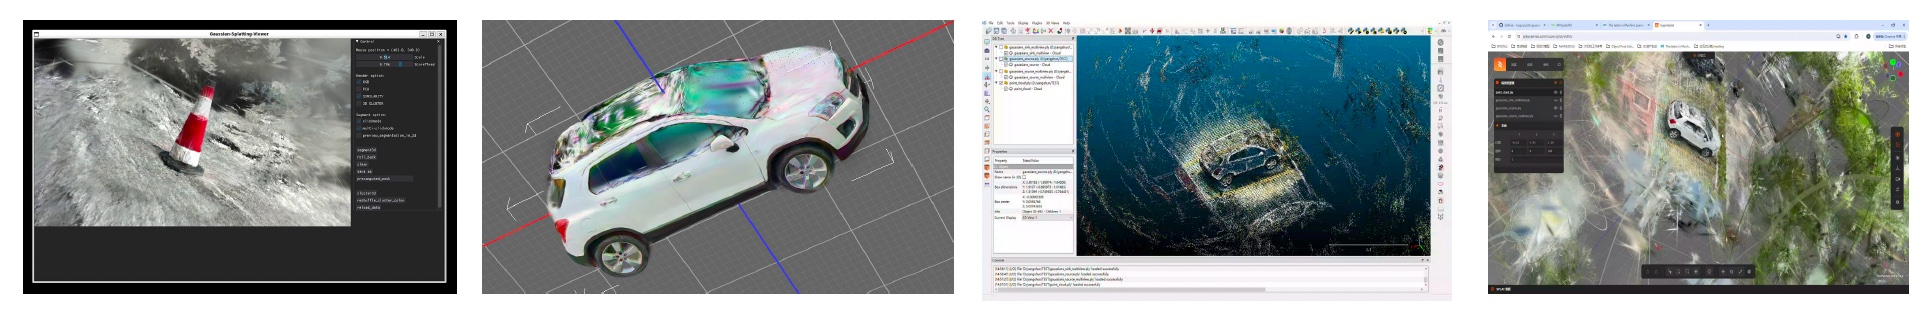
\includegraphics[width=0.95\textwidth]{imgs/gen_3d_object_to_edit.jpeg}
  \caption{3D场景重建与资产提取}
  \label{fig:gen-3d-object}
\end{figure}

\subsection{场景编辑与对象插入}

图~\ref{fig:scene-edit}展示了将重建的3D物体插入到已有场景中的效果。该功能通过在真实场景中添加、移除或修改物体,实现多样化测试场景的构建,是corner case生成的核心技术之一。

场景编辑的关键在于确保插入物体与背景场景的一致性。系统通过组合渲染管线,统一处理背景高斯、物体高斯和天空环境,正确计算遮挡关系和深度排序。通过4DGS的可微分特性,系统优化插入物体的空间变换参数,使其自然融入场景。

从图中可以观察到,插入车辆与背景场景形成了一致的视觉效果,光照匹配合理,边缘过渡自然。系统支持对插入物体进行平移、旋转和缩放等自由变换,为corner case的灵活构建提供了有效工具。场景编辑功能的实现体现了五层解耦架构的优势,系统能够独立管理背景和动态物体,支持灵活的场景组合。生成的编辑场景可有效用于自动驾驶感知和规划算法的训练测试,显著降低了数据采集成本。

\begin{figure}[htbp]
  \centering
  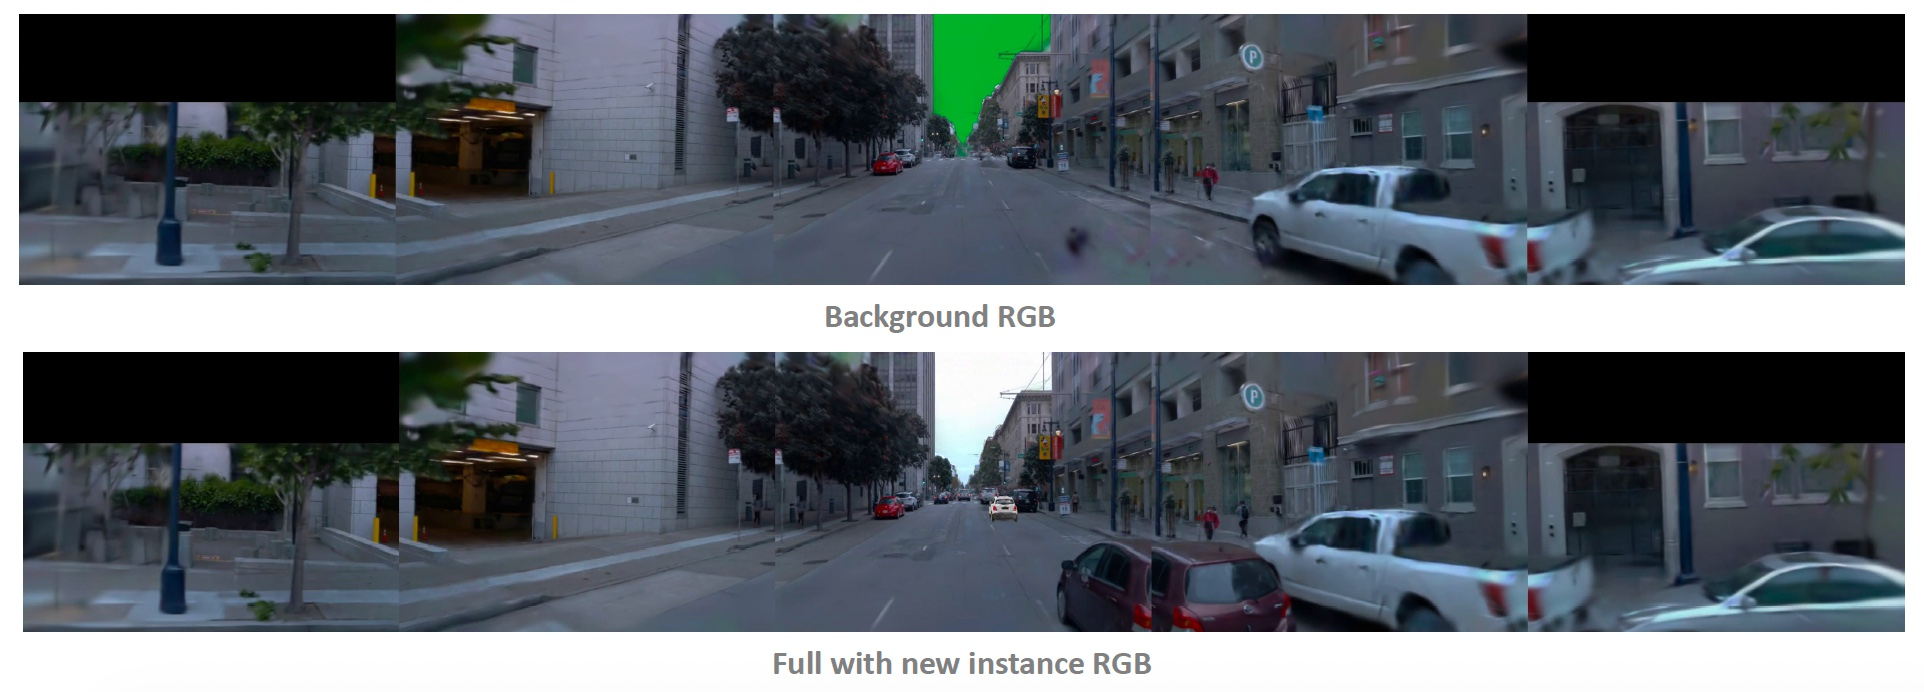
\includegraphics[width=0.95\textwidth]{imgs/3d_scen_edit_with_object.jpeg}
  \caption{场景编辑与对象插入效果}
  \label{fig:scene-edit}
\end{figure}

\subsection{扩散引导训练流程}

图~\ref{fig:training-pipeline}展示了系统从多视角图像到新视角渲染的完整流程,包括数据处理、场景表示构建、扩散引导训练和渲染输出等阶段。

训练流程以多视角图像为输入,经数据预处理生成LiDAR几何条件和相机参数,用于初始化4DGS场景表示。系统构建包含静态背景、动态物体和天空环境的完整场景模型,采用联合优化策略:在训练视点上利用真实图像进行重建损失监督,在新视点上引入扩散模型生成的伪真值进行引导训练。

图中展示的中间结果包括深度图和渲染质量评估等可视化信息。深度图验证了4DGS表示的几何准确性,扩散模型的条件引导为新视点提供了高质量监督信号,克服了传统方法在视点外推时缺乏真值的局限。训练过程采用自适应调度策略,根据模型收敛状态动态调整扩散采样频率和引导强度,确保训练稳定性。

最终渲染结果表明,系统在新视角合成任务上实现了良好的几何一致性和纹理细节。相比仅依靠训练视点监督的方法,引入扩散先验后系统在新视角外推时表现出更强的泛化能力。该流程验证了扩散引导训练策略在提升场景重建质量方面的有效性。

\begin{figure}[htbp]
  \centering
  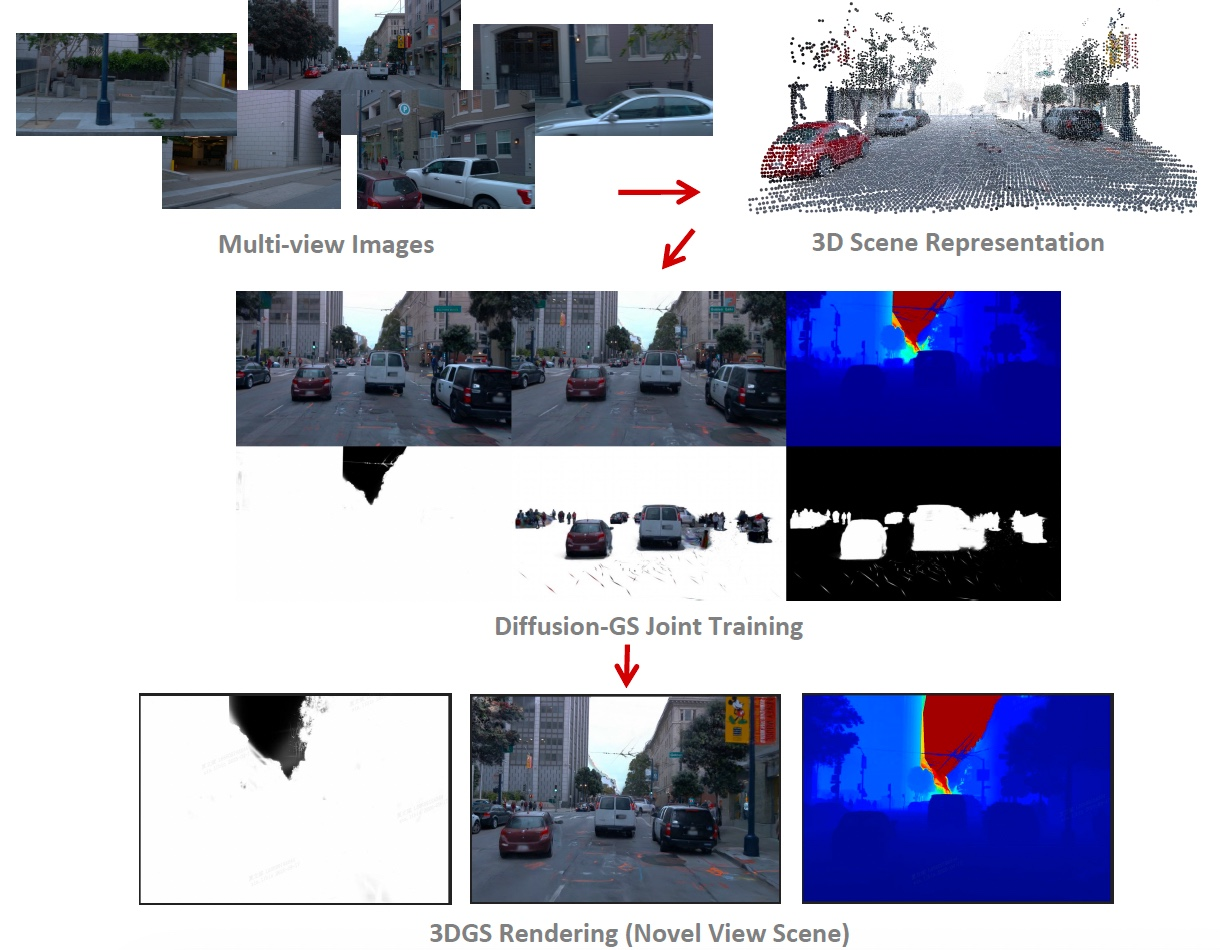
\includegraphics[width=0.95\textwidth]{imgs/from_image_train_to_rendering.jpeg}
  \caption{扩散引导训练与渲染流程}
  \label{fig:training-pipeline}
\end{figure}

\subsection{新视角合成质量对比}

图~\ref{fig:nvs-comparison}对比了不同方法在新视角合成任务上的效果,包括基线方法StreetGS、中间训练阶段结果以及最终的扩散引导方法。对比实验验证了扩散引导策略的有效性。

从对比结果可以观察到各方法的显著差异。StreetGS基线方法在新视角外推时出现明显的模糊和失真,特别是在远离训练视点的区域,图像质量下降明显,细节丢失严重。这反映了传统4DGS方法在缺乏新视点监督时的固有局限性,即过拟合于训练视点而难以泛化到未见区域。中间训练阶段的结果展示了引入扩散引导后的渐进式改善。

最终的扩散引导方法在多个评估维度上表现优异。在几何一致性方面,生成图像准确保持了场景的空间结构,建筑物轮廓清晰,透视关系正确。在纹理细节方面,图像保留了丰富的高频信息,道路标识清晰,车辆表面材质真实。在时序连贯性方面,连续帧之间过渡平滑,未出现明显闪烁或不连续现象。

定性分析表明,扩散先验的引入是质量提升的关键因素。预训练视频扩散模型包含丰富的场景先验知识,能够推理合理的场景结构和纹理细节。通过训练自由引导机制,系统将生成能力传递给4DGS模型,使其在新视点渲染时不仅依赖几何约束,还能利用先验知识进行外推。自适应采样调度策略确保了引导过程的稳定性,避免了过度依赖扩散监督导致的模型退化。对比结果验证了系统设计的有效性。

\begin{figure}[htbp]
  \centering
  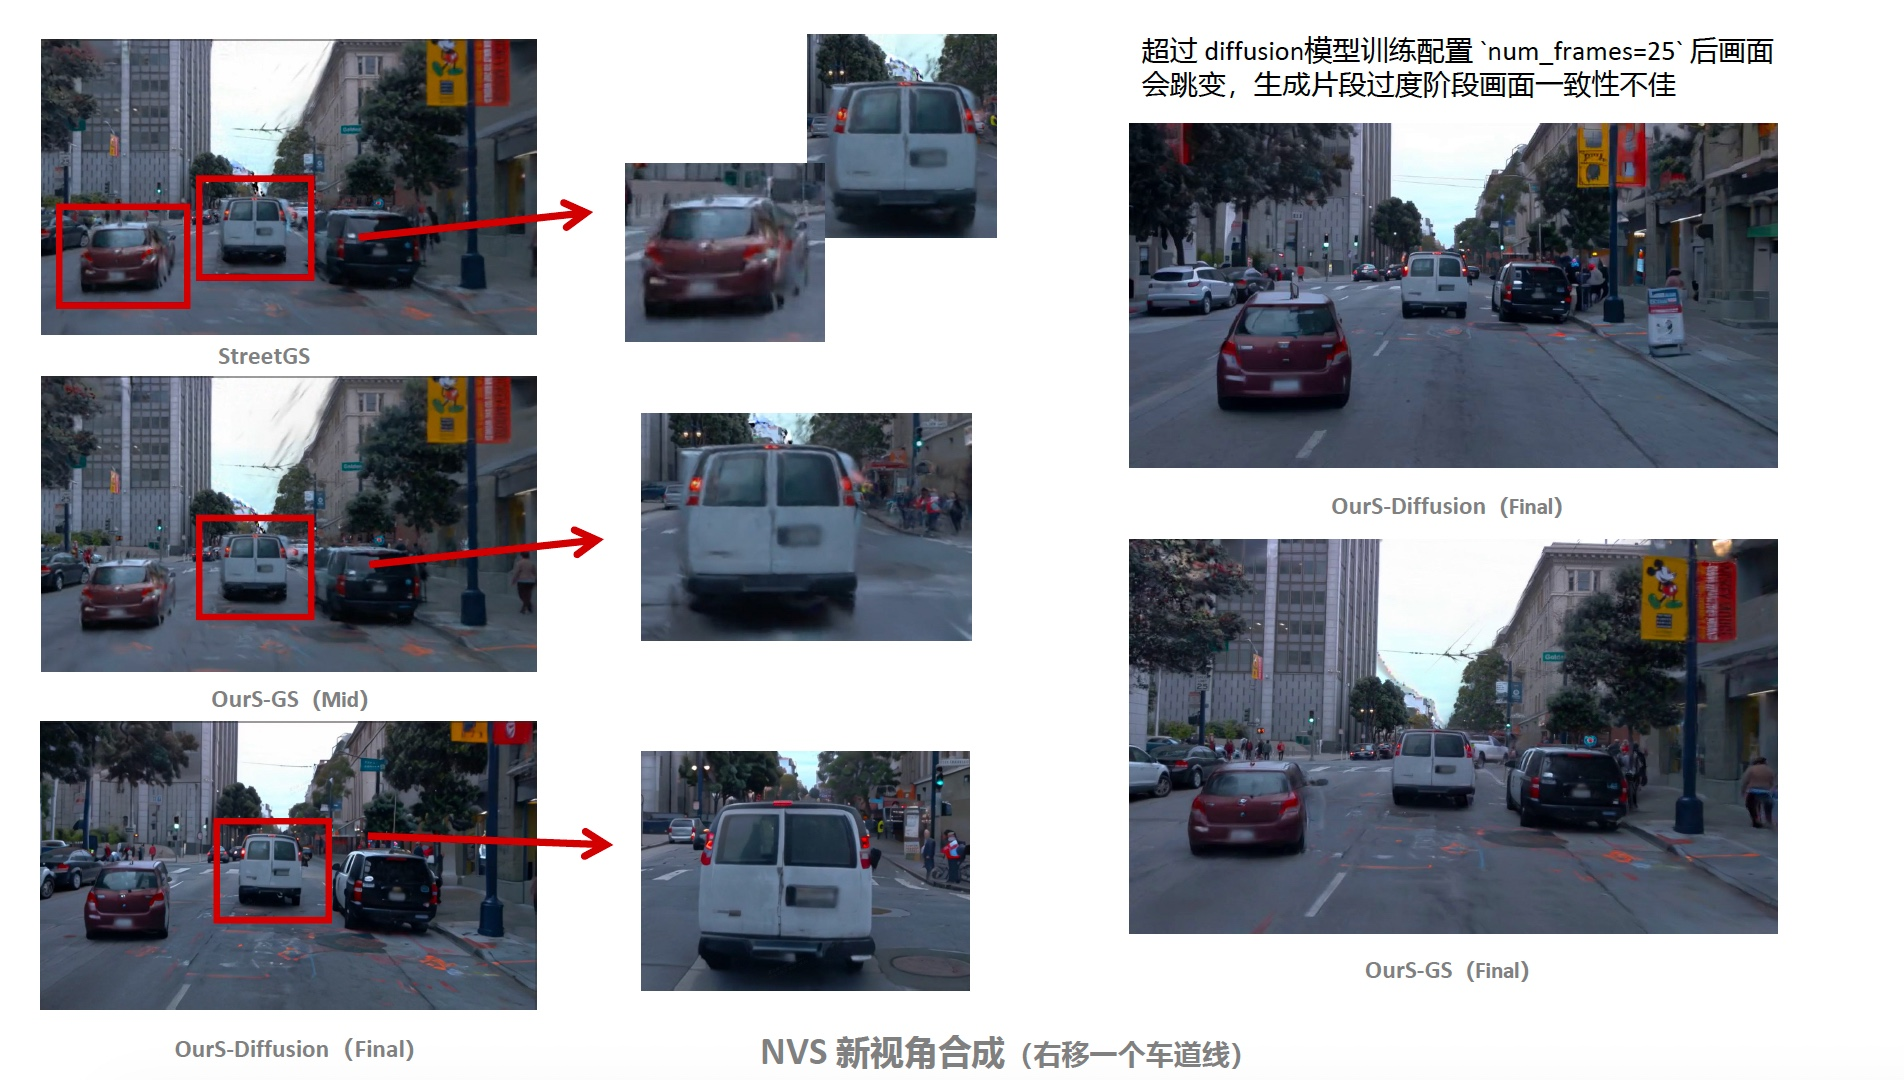
\includegraphics[width=0.95\textwidth]{imgs/nvs_compare_gs_and_diffusion_diffusiongs.jpeg}
  \caption{新视角合成质量对比}
  \label{fig:nvs-comparison}
\end{figure}

\section{本章小结}

本章从系统架构和工程实现的角度,详细阐述了ReGen系统的设计原理和关键技术实现。本文提出的五层解耦架构有效降低了系统复杂度,提高了可维护性和可扩展性。针对4D高斯溅射和视频扩散模型融合的技术挑战,系统设计了多模态渲染管线和GPU加速优化策略,实现了高性能的实时渲染。

在扩散模型集成方面,系统采用了基于Wan2.2-I2V-A14B的Diffusion Transformer架构,通过自适应采样调度和训练自由引导机制实现了高效的扩散监督训练。针对长视频序列处理的内存挑战,系统设计了滑动窗口机制和键值缓存策略,使得系统能够在单个GPU上生成长时长的高分辨率视频序列。

在系统优化方面,系统实现了分层内存管理策略和异步计算流水线,显著提升了训练效率。数值稳定性和收敛性保证机制确保了训练过程的鲁棒性。针对4DGS的动态几何表示需求,本文提出了多准则密化决策算法,综合考虑梯度统计、几何特征和时间一致性来指导高斯基元的动态调整。

在分布式训练方面,系统设计了融合FSDP和Ulysses序列并行的分布式训练架构,通过参数分片、梯度压缩和动态负载均衡策略,支持在多GPU集群上进行大规模模型的高效训练。针对不同的部署需求,系统实现了灵活的多模式推理引擎,支持各种硬件配置和应用场景。

数据处理系统实现了完整的处理管线,包括天空掩码生成、彩色点云融合和LiDAR条件图像生成。质量监控系统通过多维度指标的综合评估,确保了训练过程的稳定性和可靠性。这些系统级的工程创新为高保真4D场景重建的实际应用提供了坚实的技术基础。


% 参考文献
\bibliography{ref/refs}  % 参考文献使用 BibTeX 编译
% \printbibliography       % 参考文献使用 BibLaTeX 编译

% 附录
\appendix
% \input{data/appendix-survey}       % 本科生:外文资料的调研阅读报告
% \input{data/appendix-translation}  % 本科生:外文资料的书面翻译
% \input{data/appendix}

% 其他部分
\backmatter

% 致谢
\input{data/acknowledgements}

% 声明
% 各类开题报告通常不需要
% \statement[page-style=empty]  % 编译生成的声明页默认不含页眉页脚,以避免页码变化带来问题
% 在提交终稿时,插入签字后的扫描件 scan-statement.pdf,并添加页眉页脚
% \statement[page-style=plain, file=scan-statement.pdf]
% 如确实需要在电子版中直接页眉页脚,则使用
% \statement[page-style=plain]

% 个人简历、在学期间完成的相关学术成果
% 本科生可以附个人简历,也可以不附个人简历
\input{data/resume}

% 指导教师/指导小组评语
% 本科生不需要
\input{data/comments}

% 答辩委员会决议书
% 本科生不需要
\input{data/resolution}

% 本科生的综合论文训练记录表(扫描版)
% \record{file=scan-record.pdf}

\end{document}
